%% ============================================================
%% Differential Protection in IBR-Dominated Networks
%% Research Highlights — SAMBPS Framework
%%
%% Audience  : Senior Scientists, Protection Industry, Germany
%% Author    : Anoop V. Eluvathingal, IIT Madras
%% Supervisor: Prof. K. Shanti Swarup
%% Date      : April 2026
%%
%% Compile   : pdflatex diff_protection_germany.tex (twice)
%%
%% SPEAKER NOTES
%%   Notes are embedded in every frame using \note{...}.
%%   To produce a notes-only PDF for printing, uncomment:
%%     \setbeameroption{show only notes}
%%   To show notes alongside slides (dual monitor):
%%     \setbeameroption{show notes on second screen=right}
%%   Default (commented): slides only.
%% ============================================================
\documentclass[aspectratio=169, 10pt]{beamer}

%% ── Speaker notes ───────────────────────────────────────────
\usepackage{pgfpages}
%\setbeameroption{show only notes}            %% notes PDF for printing
%\setbeameroption{show notes on second screen=right}  %% dual monitor

%% ── Packages ────────────────────────────────────────────────
\usepackage{tikz}
\usepackage{pgfplots}
\pgfplotsset{compat=1.18}
\usetikzlibrary{%
  shapes, shapes.geometric, arrows, arrows.meta,
  calc, positioning, fit, matrix,
  decorations.pathreplacing, decorations.markings, patterns,
  overlay-beamer-styles,
}
\usepackage{amsmath, amssymb, bm}
\usepackage{booktabs}
\usepackage{array, multirow, tabularx}
\usepackage[table]{xcolor}
\usepackage{colortbl}
\usepackage{graphicx}
\usepackage{tcolorbox}
\tcbuselibrary{skins, breakable}
\usepackage{pifont}
\usepackage{siunitx}

%% ── Colour palette ──────────────────────────────────────────
\definecolor{iitmMaroon}  {RGB}{128,  0,  0}
\definecolor{iitmGold}    {RGB}{179,145, 25}
\definecolor{iitmDarkBlue}{RGB}{ 15, 45, 90}
\definecolor{iitmLightBg} {RGB}{248,244,240}
\definecolor{thesisblue}  {RGB}{  0, 70,140}
\definecolor{thesisred}   {RGB}{180, 30, 30}
\definecolor{thesisgreen} {RGB}{ 20,120, 60}
\definecolor{thesisorange}{RGB}{200, 90,  0}
\definecolor{thesisgray}  {RGB}{100,100,110}
\definecolor{thesisteal}  {RGB}{  0,130,130}
\definecolor{thesispurple}{RGB}{100,  0,150}
\definecolor{lightblue}   {RGB}{220,235,255}
\definecolor{lightgreen}  {RGB}{220,245,225}
\definecolor{lightorange} {RGB}{255,240,220}
\definecolor{lightyellow} {RGB}{255,252,220}
\definecolor{lightgray}   {RGB}{240,240,242}
\definecolor{passpink}    {RGB}{255,245,245}
\definecolor{passgreen}   {RGB}{235,252,235}

%% ── Beamer theme ────────────────────────────────────────────
\usetheme{default}
\usecolortheme[named=iitmMaroon]{structure}

\setbeamercolor{palette primary}   {bg=iitmMaroon,   fg=white}
\setbeamercolor{palette secondary} {bg=iitmMaroon,   fg=white}
\setbeamercolor{frametitle}        {bg=iitmMaroon,   fg=white}
\setbeamercolor{title}             {fg=white,        bg=iitmMaroon}
\setbeamercolor{block title}       {fg=white,        bg=iitmDarkBlue}
\setbeamercolor{block body}        {bg=iitmLightBg}
\setbeamercolor{alerted text}      {fg=iitmMaroon}
\setbeamercolor{background canvas} {bg=white}
\setbeamerfont{frametitle}{size=\large, series=\bfseries}
\setbeamerfont{title}     {size=\Large, series=\bfseries}
\setbeamertemplate{navigation symbols}{}

%% Frametitle: full-width maroon bar
\setbeamertemplate{frametitle}{%
  \nointerlineskip%
  \begin{beamercolorbox}[wd=\paperwidth,ht=0.92cm,dp=0.13cm,
                          leftskip=0.55cm,rightskip=0.4cm]{frametitle}%
    \vbox to 0.92cm{\vfil%
      \usebeamerfont{frametitle}\usebeamercolor[fg]{frametitle}%
      \insertframetitle%
    \vfil}%
  \end{beamercolorbox}%
}

%% Footline: maroon bar
\setbeamertemplate{footline}{%
  \leavevmode%
  \begin{beamercolorbox}[wd=\paperwidth,ht=0.48cm,dp=0.12cm]{palette primary}%
    \hspace{0.45cm}%
    {\scriptsize\color{white}%
      A.\,V.\,Eluvathingal \enspace|\enspace
      Differential Protection in IBR Networks \enspace|\enspace
      IIT Madras}%
    \hfill%
    {\scriptsize\color{white}%
      \insertframenumber/\inserttotalframenumber%
      \hspace{0.45cm}}%
  \end{beamercolorbox}%
}

%% ── Macros ──────────────────────────────────────────────────
\newcommand{\SAMBPS}{\textsc{sambps}}
\newcommand{\pu}{\,\text{p.u.}}
\newcommand{\ms}{\,\text{ms}}
\newcommand{\Hz}{\,\text{Hz}}
\newcommand{\kIBR}{k_{\rm ibr}}
\newcommand{\kn}{\kappa_n}
\newcommand{\cmark}{\textcolor{thesisgreen}{\ding{51}}}
\newcommand{\xmark}{\textcolor{thesisred}{\ding{55}}}
\newcommand{\PD}{P_D}
\newcommand{\PFA}{P_{FA}}

%% Result highlight box
\tcbset{
  resultbox/.style={
    enhanced, boxrule=0.8pt, arc=3pt,
    colback=passgreen, colframe=thesisgreen,
    fonttitle=\bfseries\footnotesize, coltitle=white,
    attach boxed title to top left={yshift=-2mm, xshift=3mm},
    boxed title style={colback=thesisgreen, arc=2pt},
    left=2mm, right=2mm, top=2mm, bottom=2mm,
  },
  warnbox/.style={
    enhanced, boxrule=0.8pt, arc=3pt,
    colback=lightorange, colframe=thesisorange,
    fonttitle=\bfseries\footnotesize, coltitle=white,
    attach boxed title to top left={yshift=-2mm, xshift=3mm},
    boxed title style={colback=thesisorange, arc=2pt},
    left=2mm, right=2mm, top=2mm, bottom=2mm,
  },
  keybox/.style={
    enhanced, boxrule=0.8pt, arc=3pt,
    colback=lightblue, colframe=thesisblue,
    left=2mm, right=2mm, top=1.5mm, bottom=1.5mm,
  },
}

%% ── Title metadata ──────────────────────────────────────────
\title[Differential Protection \textbar\ IBR Networks]{%
  \textbf{Differential Protection in\\
  Inverter-Based Resource Dominated Networks}\\[4pt]
  {\large Research Highlights — \SAMBPS{} Framework}}

\author[A.\,V.\,Eluvathingal \& K.\,S.\,Swarup]{%
  \textbf{Anoop V.\ Eluvathingal}\quad|\quad
  Supervisor: Prof.\ K.\ Shanti Swarup\\[2pt]
  {\small Department of Electrical Engineering,
    Indian Institute of Technology Madras, Chennai~600\,036, India}}

\date{April 2026}

%% ============================================================
\begin{document}
%% ============================================================

%% ── Title slide ─────────────────────────────────────────────
{%
\setbeamertemplate{footline}{}
\begin{frame}[plain]
  \begin{tikzpicture}[overlay, remember picture]
    \fill[iitmMaroon]
      (current page.north west) rectangle
      ([yshift=-3.6cm]current page.north east);
    \node[anchor=center, text=white, align=center, font=\Large\bfseries,
          text width=14cm]
      at ([yshift=-1.4cm]current page.north)
      {Differential Protection in\\
       Inverter-Based Resource Dominated Networks};
    \fill[iitmGold]
      ([yshift=-3.6cm]current page.north west) rectangle
      ([yshift=-3.9cm]current page.north east);
  \end{tikzpicture}
\note{
  Welcome and introduce yourself: PhD candidate at IIT Madras, working on
  adaptive protection for inverter-dominated networks under Prof.\ Swarup.
  Emphasise that this talk targets the \emph{differential protection} subset
  of the broader SAMBPS framework --- 87T, 87L, and 87B --- with full
  Monte Carlo and hardware-in-the-loop validation results.
  Expected duration: 35--40 minutes plus 10 minutes discussion.
}
\end{frame}
}

%% ── Outline ─────────────────────────────────────────────────
\begin{frame}{Presentation Outline}
\vspace{2pt}
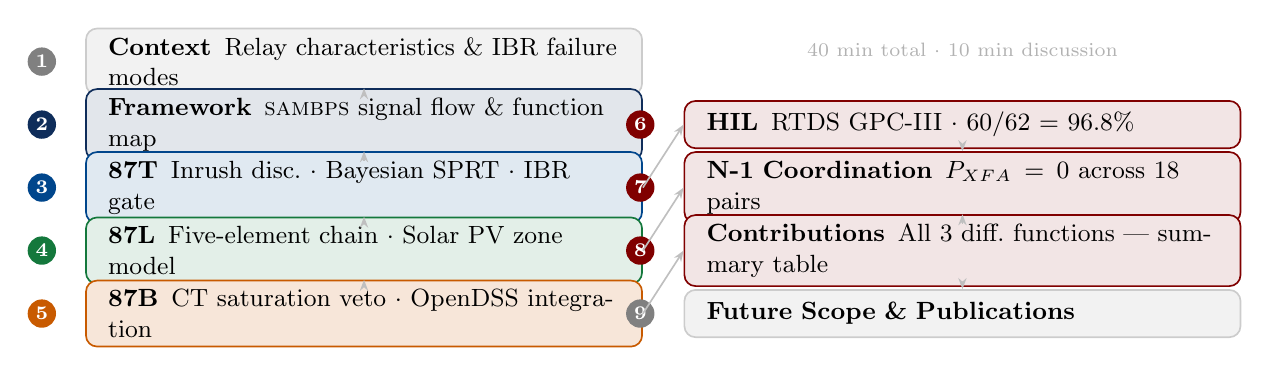
\begin{tikzpicture}[
  sec/.style={rectangle, rounded corners=4pt, minimum height=0.60cm,
    text width=6.5cm, align=left, inner xsep=8pt, font=\small,
    line width=0.6pt},
  dot/.style={circle, minimum size=0.36cm, inner sep=0pt,
    font=\bfseries\scriptsize, text=white},
  arr/.style={-{Stealth[length=4pt]}, gray!50, line width=0.6pt},
]
%% Column 1 — left
\node[sec, fill=gray!10, draw=gray!40]           (S1) at (0, 0)
  {\textbf{Context}\enspace Relay characteristics \& IBR failure modes};
\node[sec, fill=iitmDarkBlue!12, draw=iitmDarkBlue] (S2) at (0,-0.80)
  {\textbf{Framework}\enspace \SAMBPS{} signal flow \& function map};
\node[sec, fill=thesisblue!12, draw=thesisblue]  (S3) at (0,-1.60)
  {\textbf{87T}\enspace Inrush disc.\ $\cdot$ Bayesian SPRT $\cdot$ IBR gate};
\node[sec, fill=thesisgreen!12, draw=thesisgreen] (S4) at (0,-2.40)
  {\textbf{87L}\enspace Five-element chain $\cdot$ Solar PV zone model};
\node[sec, fill=thesisorange!15, draw=thesisorange](S5) at (0,-3.20)
  {\textbf{87B}\enspace CT saturation veto $\cdot$ OpenDSS integration};

%% Column 2 — right
\node[sec, fill=iitmMaroon!10, draw=iitmMaroon]  (S6) at (7.6,-0.80)
  {\textbf{HIL}\enspace RTDS GPC-III $\cdot$ 60/62 = 96.8\%};
\node[sec, fill=iitmMaroon!10, draw=iitmMaroon]  (S7) at (7.6,-1.60)
  {\textbf{N-1 Coordination}\enspace $P_{XFA}=0$ across 18 pairs};
\node[sec, fill=iitmMaroon!10, draw=iitmMaroon]  (S8) at (7.6,-2.40)
  {\textbf{Contributions}\enspace All 3 diff.\ functions — summary table};
\node[sec, fill=gray!10, draw=gray!40]            (S9) at (7.6,-3.20)
  {\textbf{Future Scope \& Publications}};

%% Badges
\foreach \n/\nd/\col in {
  1/S1/gray,2/S2/iitmDarkBlue,3/S3/thesisblue,
  4/S4/thesisgreen,5/S5/thesisorange}{
  \node[dot, fill=\col] at ([xshift=-0.55cm]\nd.west) {\n};
}
\foreach \n/\nd/\col in {
  6/S6/iitmMaroon,7/S7/iitmMaroon,8/S8/iitmMaroon,9/S9/gray}{
  \node[dot, fill=\col] at ([xshift=-0.55cm]\nd.west) {\n};
}

%% Connector arrows between columns
\draw[arr] (S3.east) -- (S6.west);
\draw[arr] (S4.east) -- (S7.west);
\draw[arr] (S5.east) -- (S8.west);

%% Vertical flow arrows left column
\foreach \a/\b in {S1/S2, S2/S3, S3/S4, S4/S5}{
  \draw[arr] (\a.south) -- (\b.north);
}
\foreach \a/\b in {S6/S7, S7/S8, S8/S9}{
  \draw[arr] (\a.south) -- (\b.north);
}

%% Duration label
\node[font=\scriptsize, text=gray!60] at (7.6, 0.15)
  {40 min total $\cdot$ 10 min discussion};
\end{tikzpicture}
\note{
  Walk the audience through the structure.
  Parts 2--4 can be presented in any order if time is short ---
  the function map (slide 5) makes dependencies visible.
  Recommended cuts for a 25-minute version: omit N-1 slide and
  compress TR-64 integration into the SPRT slide.
  The HIL slide is non-negotiable for an industrial audience.
}
\end{frame}

%%=============================================================
%% CONVENTIONAL RELAY SETTINGS — THREE-PANEL OVERVIEW
%%=============================================================

\begin{frame}{Conventional Differential Relay Characteristics — 87T / 87L / 87B}
\vspace{-2pt}
%% ── shared pgfplot style (panel dims tuned for 16:9 slide) ─────────────────
\pgfplotsset{
  diffchar/.style={
    width=4.25cm, height=3.55cm,
    scale only axis,
    xmin=0, xmax=4.0, ymin=0,
    grid=both, grid style={gray!20, line width=0.2pt},
    minor tick num=0,
    xtick={0,1,2,3,4},
    tick label style={font=\tiny},
    label style={font=\tiny},
    title style={font=\small\bfseries, color=iitmDarkBlue, yshift=2pt},
    legend style={font=\tiny, inner sep=2pt, row sep=-2pt,
                  fill=white, draw=black!25, line width=0.3pt},
    every axis plot/.append style={line width=0.75pt},
    xlabel style={yshift=2pt},
    ylabel style={yshift=-4pt},
  }
}
\begin{columns}[c]

%% ══════════════════════════════════════════════════════════════════════════════
\column{0.333\textwidth}
\centering
\begin{tikzpicture}
\begin{axis}[
  diffchar,
  ymax=2.6,
  ytick={0,0.5,1.0,1.5,2.0,2.5},
  xlabel={$I_{rst}$ [pu]},
  ylabel={$I_{op}$ [pu]},
  title={87T — Transformer Differential},
  legend pos=north west,
]
  \addplot[red!10, fill=red!8, draw=none, forget plot]
    coordinates {(0,0.20)(1.0,0.25)(4.0,2.05)(4.0,2.6)(0,2.6)(0,0.20)};
  \addplot[green!8, fill=green!6, draw=none, forget plot]
    coordinates {(0,0)(4.0,0)(4.0,2.05)(1.0,0.25)(0,0.20)(0,0)};
  \addplot[red, thick, domain=0:1.0, samples=40]
    { max(0.20, 0.25*x) };
  \addlegendentry{SLP1=0.25 / SLP2=0.60};
  \addplot[red, thick, domain=1.0:4.0, samples=40, forget plot]
    { 0.25 + 0.60*(x-1.0) };
  \addplot[gray!60, dashed, thin, domain=0:4.0, forget plot] {0.20};
  \addplot[thesispurple, dashed, thin, domain=0:4.0, forget plot] {2.50};
  \node[font=\tiny, red!80!black] at (axis cs:0.5,0.09) {SLP1};
  \node[font=\tiny, red!80!black, rotate=40] at (axis cs:2.1,1.20) {SLP2};
  \node[font=\tiny, gray!65] at (axis cs:2.9,0.27) {$I_{op,\min}$};
  \node[font=\tiny, thesispurple] at (axis cs:2.2,2.57) {High-set};
  \node[font=\tiny\bfseries, red!65!black]   at (axis cs:2.8,2.20) {TRIP};
  \node[font=\tiny\bfseries, green!55!black] at (axis cs:2.2,0.10) {RESTRAIN};
  \draw[dashed, gray!35, very thin] (axis cs:1.0,0) -- (axis cs:1.0,0.25);
\end{axis}
\end{tikzpicture}

%% ══════════════════════════════════════════════════════════════════════════════
\column{0.333\textwidth}
\centering
\begin{tikzpicture}
\begin{axis}[
  diffchar,
  ymax=1.05,
  ytick={0,0.2,0.4,0.6,0.8,1.0},
  xlabel={$I_{\rm rest}$ [pu]},
  ylabel={$I_{\rm thr}$ [pu]},
  title={87L — Line Current Differential},
  legend pos=north west,
]
  %% IBR failure zone
  \addplot[red!15, fill=red!12, draw=none, forget plot]
    coordinates {(0,0.06)(4.0,0.06)(4.0,0.20)(0,0.20)(0,0.06)};
  \node[font=\tiny, red!65!black, align=center]
    at (axis cs:2.9,0.13) {\textbf{IBR fail zone}};
  %% SAMBPS recovery fill
  \addplot[blue!7, fill=blue!6, draw=none, forget plot, domain=0:4.0]
    { max(0.20, 0.25*x) } \closedcycle;
  \addplot[white, fill=white, draw=none, forget plot, domain=0:4.0]
    { max(0.08, 0.15*x) } \closedcycle;
  %% Conventional
  \addplot[red, thick, domain=0:4.0, samples=60]
    { max(0.20, 0.25*x) };
  \addlegendentry{Conv.: $\max(0.20,\;0.25I)$};
  %% SAMBPS adaptive
  \addplot[thesisblue, thick, domain=0:4.0, samples=60]
    { max(0.08, 0.15*x) };
  \addlegendentry{SAMBPS: $\max(0.08,\;0.15I)$};
  %% CT error
  \addplot[gray!55, dotted, thin, domain=0:4.0, forget plot] { 0.005*x };
  %% Region labels
  \node[font=\tiny\bfseries, red!65!black]   at (axis cs:1.0,0.78) {TRIP (both)};
  \node[font=\tiny\bfseries, thesisblue]     at (axis cs:2.6,0.44) {SAMBPS};
  \node[font=\tiny\bfseries, green!55!black] at (axis cs:2.5,0.025) {RESTRAIN};
  %% Knee points
  \draw[dashed, gray!40, very thin] (axis cs:0.80,0) -- (axis cs:0.80,0.20);
  \draw[dashed, gray!40, very thin] (axis cs:0.53,0) -- (axis cs:0.53,0.08);
\end{axis}
\end{tikzpicture}

%% ══════════════════════════════════════════════════════════════════════════════
\column{0.333\textwidth}
\centering
\begin{tikzpicture}
\begin{axis}[
  diffchar,
  ymax=5.0,
  ytick={0,1,2,3,4,5},
  xlabel={$I_{rst}$ [pu]},
  ylabel={$I_{op}$ [pu]},
  title={87B — Busbar Differential},
  legend pos=north west,
]
  \addplot[green!8, fill=green!6, draw=none, forget plot]
    coordinates {(0,0)(4.0,0)(4.0,2.0)(1.0,0.25)(0,0.20)(0,0)};
  \addplot[thesisorange, thick, domain=0:1.0, samples=40]
    { max(0.20, 0.25*x) };
  \addlegendentry{SLP1=0.25 / SLP2=0.50};
  \addplot[thesisorange, thick, domain=1.0:4.0, samples=40, forget plot]
    { 0.25 + 0.50*(x-1.0) };
  \addplot[gray!60, dashed, thin, domain=0:4.0, forget plot] {0.20};
  \node[font=\tiny, thesisorange!85!black] at (axis cs:0.5,0.09) {SLP1};
  \node[font=\tiny, thesisorange!85!black, rotate=28] at (axis cs:2.2,1.10) {SLP2};
  \addplot[only marks, mark=triangle*, mark size=2.8pt, thesisorange!80!red]
    coordinates {(2.5, 4.65)};
  \addlegendentry{CT-sat (VETOED)};
  \node[font=\tiny, thesisorange!80!red] at (axis cs:3.5,4.65) {\textbf{VETO}};
  \addplot[only marks, mark=star, mark size=3pt, red]
    coordinates {(1.5, 3.0)};
  \addlegendentry{Internal (TRIP)};
  \addplot[only marks, mark=square*, mark size=2pt, thesisgreen]
    coordinates {(2.5, 0.0)};
  \addlegendentry{External (RESTRAIN)};
  \node[font=\tiny\bfseries, thesisorange!80!black] at (axis cs:2.8,3.6) {TRIP};
  \node[font=\tiny\bfseries, green!55!black] at (axis cs:2.5,0.12) {RESTRAIN};
  \draw[dashed, gray!35, very thin] (axis cs:1.0,0) -- (axis cs:1.0,0.25);
\end{axis}
\end{tikzpicture}

\end{columns}

\vspace{4pt}
\begin{tcolorbox}[enhanced, boxrule=0.5pt, arc=2pt,
  colback=iitmLightBg, colframe=thesisgray,
  left=4pt, right=4pt, top=1.5pt, bottom=1.5pt]
{\tiny
\textbf{87T:} Dual-slope boundary; inrush/IBR-fault discrimination not solvable by slope alone.\quad
\textbf{87L \textcolor{red!70!black}{(red zone)}:} IBR fault $I_{\rm diff}=0.06$--$0.20$\,p.u.\ falls below conventional pickup — relay fails.\quad
\textbf{87B \textcolor{thesisorange!80!red}{(orange $\blacktriangle$)}:} CT saturation inflates $I_{op}$; SAMBPS Stage-2 veto correctly blocks trip.
}
\end{tcolorbox}
\note{
  Use this slide as the motivating evidence before introducing SAMBPS.
  The three panels share the same $I_{rst}$/$I_{op}$ axes so the audience
  can compare directly across functions.\\[4pt]
  Key talking point per panel:
  \begin{itemize}
    \item \textbf{87T}: dual-slope is standard (IEC\,60255-121); the problem
      is not the shape but the inrush/IBR-fault discrimination that slope
      alone cannot solve.
    \item \textbf{87L}: the red zone ($0.06$--$0.20$\,p.u.) is exactly where
      IBR fault current lands.  The conventional relay is blind here.
      SAMBPS lowers the floor from 0.20 to 0.08\,p.u.\ and reduces the slope
      from 0.25 to 0.15 while maintaining a 30$\times$ CT margin.
    \item \textbf{87B}: the orange triangle is the CT-saturation scenario
      where conventional 87B would nuisance-trip; SAMBPS Stage-2 veto
      correctly blocks it.  The restrain/trip boundary itself is unchanged
      --- only the Stage-2 gate is new.
  \end{itemize}
}
\end{frame}

%%=============================================================
%% PART 1 — FRAMEWORK
%%=============================================================

\begin{frame}{The IBR Protection Problem — Why Conventional Relays Fail}
\vspace{-2pt}
\begin{center}
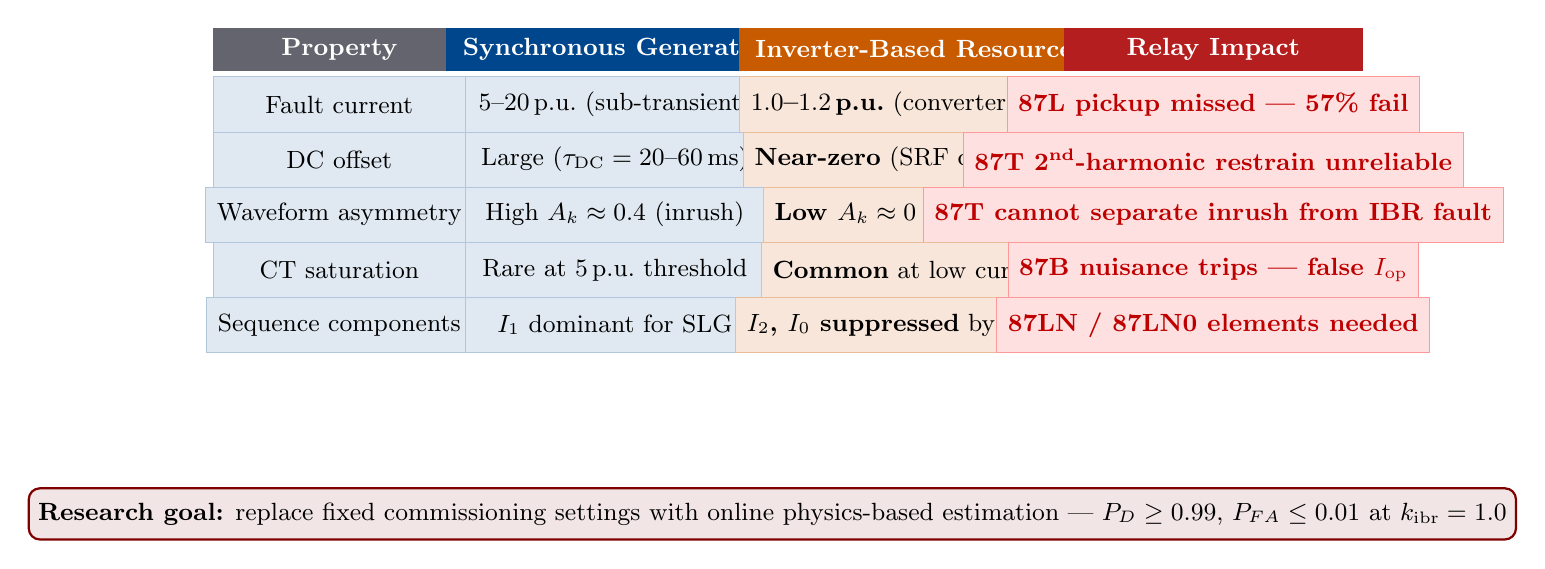
\begin{tikzpicture}[
  hdr/.style={rectangle, minimum height=0.55cm, align=center,
    font=\small\bfseries, text=white, inner xsep=6pt},
  cel/.style={rectangle, minimum height=0.70cm, align=center,
    font=\small, inner xsep=4pt, line width=0.3pt},
  sg/.style={cel, fill=thesisblue!12,  draw=thesisblue!30},
  ibr/.style={cel, fill=thesisorange!15, draw=thesisorange!40},
  fail/.style={cel, fill=red!12, draw=red!40, text=red!75!black, font=\small\bfseries},
]
%% Column widths: property=3.2cm, SG=3.8cm, IBR=3.8cm, impact=3.8cm
\def\wP{3.2} \def\wS{3.8} \def\wI{3.8} \def\wF{3.8}
\def\xs{3.2}          % x start of SG col
\def\xi{7.0}          % x start of IBR col
\def\xf{10.8}         % x start of FAIL col
\def\rh{0.70}         % row height
\def\hh{0.60}         % header height

%% ── Header row ──────────────────────────────────────────────────────────────
\node[hdr, fill=thesisgray,    minimum width=\wP cm] at (1.6,   0) {Property};
\node[hdr, fill=thesisblue,    minimum width=\wS cm] at (5.1,   0) {Synchronous Generator};
\node[hdr, fill=thesisorange,  minimum width=\wI cm] at (8.9,   0) {Inverter-Based Resource};
\node[hdr, fill=thesisred,     minimum width=\wF cm] at (12.7,  0) {Relay Impact};

%% ── Data rows ───────────────────────────────────────────────────────────────
%% row helper: y offset from top header
%% Row 1 — Fault current
\def\ry{-\rh}
\node[sg,  minimum width=\wP cm] at (1.6,  \ry) {Fault current};
\node[sg,  minimum width=\wS cm] at (5.1,  \ry) {$5$--$20\,\text{p.u.}$ (sub-transient)};
\node[ibr, minimum width=\wI cm] at (8.9,  \ry) {\textbf{$1.0$--$1.2\,\text{p.u.}$} (converter limit)};
\node[fail,minimum width=\wF cm] at (12.7, \ry) {87L pickup missed — 57\% fail};

%% Row 2 — DC offset
\def\ry{-2*\rh}
\node[sg,  minimum width=\wP cm] at (1.6,  \ry) {DC offset};
\node[sg,  minimum width=\wS cm] at (5.1,  \ry) {Large ($\tau_{\rm DC}=20$--$60\,$ms)};
\node[ibr, minimum width=\wI cm] at (8.9,  \ry) {\textbf{Near-zero} (SRF controller)};
\node[fail,minimum width=\wF cm] at (12.7, \ry) {87T 2$^\text{nd}$-harmonic restrain unreliable};

%% Row 3 — Symmetry
\def\ry{-3*\rh}
\node[sg,  minimum width=\wP cm] at (1.6,  \ry) {Waveform asymmetry};
\node[sg,  minimum width=\wS cm] at (5.1,  \ry) {High $A_k \approx 0.4$ (inrush)};
\node[ibr, minimum width=\wI cm] at (8.9,  \ry) {\textbf{Low $A_k \approx 0$} (sinusoidal)};
\node[fail,minimum width=\wF cm] at (12.7, \ry) {87T cannot separate inrush from IBR fault};

%% Row 4 — CT saturation
\def\ry{-4*\rh}
\node[sg,  minimum width=\wP cm] at (1.6,  \ry) {CT saturation};
\node[sg,  minimum width=\wS cm] at (5.1,  \ry) {Rare at $5\,$p.u.\ threshold};
\node[ibr, minimum width=\wI cm] at (8.9,  \ry) {\textbf{Common} at low current};
\node[fail,minimum width=\wF cm] at (12.7, \ry) {87B nuisance trips — false $I_{\rm op}$};

%% Row 5 — Sequence components
\def\ry{-5*\rh}
\node[sg,  minimum width=\wP cm] at (1.6,  \ry) {Sequence components};
\node[sg,  minimum width=\wS cm] at (5.1,  \ry) {$I_1$ dominant for SLG};
\node[ibr, minimum width=\wI cm] at (8.9,  \ry) {\textbf{$I_2$, $I_0$ suppressed} by control};
\node[fail,minimum width=\wF cm] at (12.7, \ry) {87LN / 87LN0 elements needed};

%% ── Research question banner ────────────────────────────────────────────────
\node[rectangle, rounded corners=4pt, line width=0.8pt,
      fill=iitmMaroon!10, draw=iitmMaroon,
      minimum width=14.2cm, minimum height=0.65cm,
      align=center, font=\small]
  at (7.1, -5.9)
  {\textbf{Research goal:} replace fixed commissioning settings with online
   physics-based estimation — $\PD \geq 0.99$, $\PFA \leq 0.01$
   at $\kIBR = 1.0$};

\end{tikzpicture}
\end{center}
\note{
  The table replaces intuition with evidence: each row is a specific,
  measurable difference between SG and IBR fault signatures, and the
  rightmost column names the specific relay element that fails as a result.
  The 57\% failure rate for 87L is from our own 21-scenario study, not
  a literature estimate.
  The IBR current limit is mandated by IEEE\,1547-2018 / IEC\,61727 ---
  relay algorithms were frozen before that standard existed.
  The core problem is fixed-parameter commissioning, not relay firmware.
  SAMBPS replaces that assumption with online inverse estimation.\\[4pt]
  Likely question: ``Can this coexist with existing IED firmware?''
  Answer: yes --- SAMBPS runs as an external IED over IEC\,61850 GOOSE.
}
\end{frame}

%% ── SAMBPS Five-Layer Architecture — Signal Flow Diagram ────
\begin{frame}{\SAMBPS{} — Signal Flow Through the Five-Layer Architecture}
\vspace{-4pt}
\begin{center}
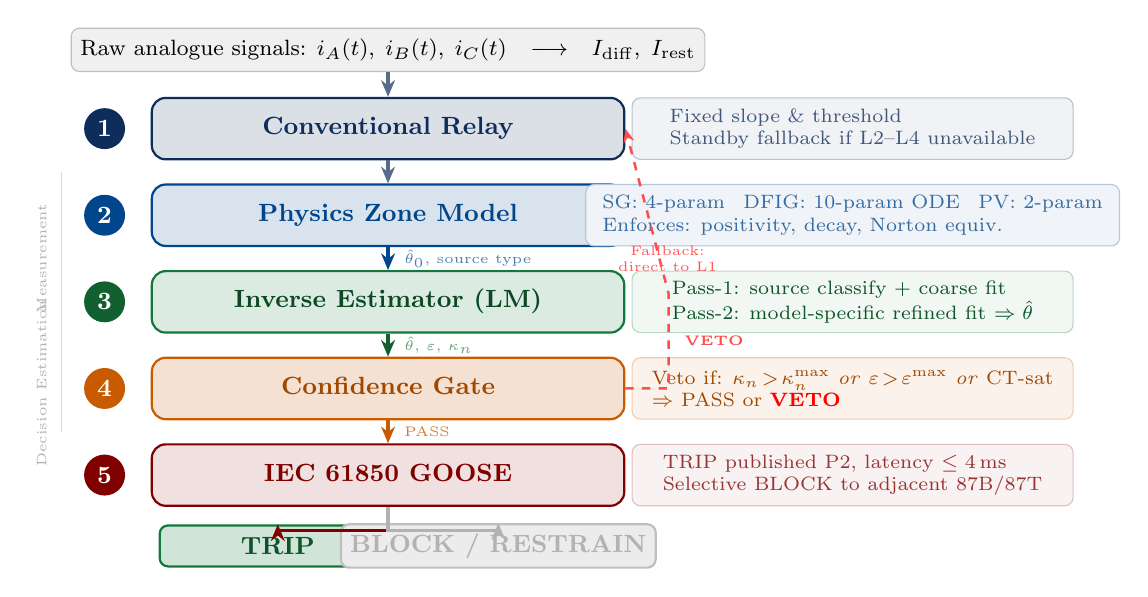
\begin{tikzpicture}[
  %% Layer block style
  blk/.style={
    rectangle, rounded corners=5pt,
    minimum width=6.0cm, minimum height=0.78cm,
    align=center, font=\small\bfseries,
    line width=0.8pt, inner sep=4pt
  },
  %% Function tag on right
  tag/.style={
    rectangle, rounded corners=3pt,
    minimum width=5.6cm, minimum height=0.78cm,
    align=left, font=\scriptsize, inner xsep=6pt,
    line width=0.4pt
  },
  %% Main flow arrow
  farr/.style={-{Stealth[length=6pt,width=5pt]}, line width=1.2pt},
  %% Feedback arrow
  barr/.style={-{Stealth[length=5pt,width=4pt]}, line width=0.9pt, dashed},
  %% Layer number badge
  badge/.style={circle, minimum size=0.52cm,
    font=\bfseries\small, inner sep=0pt},
]

%% ── Y positions (top to bottom) ────────────────────────────────────────────
%% Input, L1, L2, L3, L4, L5, Output
\def\yIN{3.2}
\def\yA{2.2}   % Layer 1
\def\yB{1.1}   % Layer 2
\def\yC{0.0}   % Layer 3
\def\yD{-1.1}  % Layer 4
\def\yE{-2.2}  % Layer 5
\def\yOUT{-3.1}

%% ── INPUT ──────────────────────────────────────────────────────────────────
\node[rectangle, rounded corners=3pt, fill=gray!12, draw=gray!50,
      minimum width=6.0cm, minimum height=0.55cm, font=\footnotesize]
  (IN) at (0,\yIN)
  {Raw analogue signals: $i_A(t),\;i_B(t),\;i_C(t)$\quad
   $\longrightarrow$\quad$I_{\rm diff},\;I_{\rm rest}$};

%% ── LAYER 1 ─────────────────────────────────────────────────────────────────
\node[blk, fill=iitmDarkBlue!15, draw=iitmDarkBlue, text=iitmDarkBlue]
  (L1) at (0,\yA) {\strut Conventional Relay};
\node[tag, fill=iitmDarkBlue!6, draw=iitmDarkBlue!30, text=iitmDarkBlue!80]
  at (5.9,\yA) {Fixed slope \& threshold\\ Standby fallback if L2--L4 unavailable};
\node[badge, fill=iitmDarkBlue, text=white] at (-3.6,\yA) {1};

%% ── LAYER 2 ─────────────────────────────────────────────────────────────────
\node[blk, fill=thesisblue!15, draw=thesisblue, text=thesisblue]
  (L2) at (0,\yB) {\strut Physics Zone Model};
\node[tag, fill=thesisblue!6, draw=thesisblue!30, text=thesisblue!80]
  at (5.9,\yB)
  {SG: 4-param \enspace DFIG: 10-param ODE \enspace PV: 2-param\\
   Enforces: positivity, decay, Norton equiv.};
\node[badge, fill=thesisblue, text=white] at (-3.6,\yB) {2};

%% ── LAYER 3 ─────────────────────────────────────────────────────────────────
\node[blk, fill=thesisgreen!15, draw=thesisgreen, text=thesisgreen!60!black]
  (L3) at (0,\yC) {\strut Inverse Estimator (LM)};
\node[tag, fill=thesisgreen!6, draw=thesisgreen!30, text=thesisgreen!70!black]
  at (5.9,\yC)
  {Pass-1: source classify $+$ coarse fit\\
   Pass-2: model-specific refined fit $\Rightarrow\hat{\theta}$};
\node[badge, fill=thesisgreen!80!black, text=white] at (-3.6,\yC) {3};

%% ── LAYER 4 ─────────────────────────────────────────────────────────────────
\node[blk, fill=thesisorange!18, draw=thesisorange, text=thesisorange!80!black]
  (L4) at (0,\yD) {\strut Confidence Gate};
\node[tag, fill=thesisorange!8, draw=thesisorange!30, text=thesisorange!80!black]
  at (5.9,\yD)
  {Veto if: $\kappa_n\!>\!\kappa_n^{\max}$ \emph{or}
   $\varepsilon\!>\!\varepsilon^{\max}$ \emph{or} CT-sat\\
   $\Rightarrow$ PASS or \textcolor{red}{\textbf{VETO}}};
\node[badge, fill=thesisorange, text=white] at (-3.6,\yD) {4};

%% ── LAYER 5 ─────────────────────────────────────────────────────────────────
\node[blk, fill=iitmMaroon!12, draw=iitmMaroon, text=iitmMaroon]
  (L5) at (0,\yE) {\strut IEC 61850 GOOSE};
\node[tag, fill=iitmMaroon!5, draw=iitmMaroon!25, text=iitmMaroon!80]
  at (5.9,\yE)
  {TRIP published P2, latency $\leq 4\,$ms\\
   Selective BLOCK to adjacent 87B/87T};
\node[badge, fill=iitmMaroon, text=white] at (-3.6,\yE) {5};

%% ── OUTPUT ──────────────────────────────────────────────────────────────────
\node[rectangle, rounded corners=3pt, line width=0.8pt,
      minimum width=3.0cm, minimum height=0.52cm, font=\small\bfseries,
      fill=thesisgreen!20, draw=thesisgreen, text=thesisgreen!70!black]
  (TRIP) at (-1.4,\yOUT) {TRIP};
\node[rectangle, rounded corners=3pt, line width=0.8pt,
      minimum width=3.0cm, minimum height=0.52cm, font=\small\bfseries,
      fill=gray!15, draw=gray!50, text=gray!60]
  (BLOCK) at (1.4,\yOUT) {BLOCK / RESTRAIN};

%% ── MAIN SIGNAL FLOW (downward) ─────────────────────────────────────────────
\draw[farr, color=iitmDarkBlue!70]
  (IN.south) -- (L1.north);
\draw[farr, color=iitmDarkBlue!70]
  (L1.south) -- (L2.north);
\draw[farr, color=thesisblue]
  (L2.south) -- (L3.north)
  node[midway, right=2pt, font=\tiny, text=thesisblue!70]
    {$\hat{\theta}_0$, source type};
\draw[farr, color=thesisgreen!80!black]
  (L3.south) -- (L4.north)
  node[midway, right=2pt, font=\tiny, text=thesisgreen!70]
    {$\hat{\theta}$, $\varepsilon$, $\kappa_n$};
\draw[farr, color=iitmMaroon]
  (L5.south) -- ++(0,-0.3) -| (TRIP.north);
\draw[farr, color=gray!60]
  (L5.south) -- ++(0,-0.3) -| (BLOCK.north);

%% ── GATE PASS PATH ──────────────────────────────────────────────────────────
\draw[farr, color=thesisorange]
  (L4.south) -- (L5.north)
  node[midway, right=2pt, font=\tiny, text=thesisorange!80]
    {PASS};

%% ── VETO FEEDBACK (right side, red dashed) ──────────────────────────────────
\draw[barr, color=red!70]
  (L4.east) -- ++(0.55,0) -- ++(0, 1.20)
  node[midway, right=2pt, font=\tiny\bfseries, text=red!70]
    {VETO}
  -- (L1.east);

%% ── FALLBACK label ──────────────────────────────────────────────────────────
\node[font=\tiny, text=red!65, align=center]
  at (3.55, 0.55) {Fallback:\\direct to L1};

%% ── LEFT LABELS ─────────────────────────────────────────────────────────────
\node[font=\tiny, text=gray!60, rotate=90, align=center]
  at (-4.4, 0.55) {Measurement};
\node[font=\tiny, text=gray!60, rotate=90, align=center]
  at (-4.4, -0.55) {Estimation};
\node[font=\tiny, text=gray!60, rotate=90, align=center]
  at (-4.4, -1.65) {Decision};
\draw[gray!30, line width=0.4pt]
  (-4.15, 1.65) -- (-4.15, -0.55);
\draw[gray!30, line width=0.4pt]
  (-4.15, -0.55) -- (-4.15, -1.65);

\end{tikzpicture}
\end{center}
\note{
  This is the architectural core of the thesis.
  The five-layer pattern was deliberately designed so that the
  \emph{same code structure} handles every protection function ---
  protection engineers can audit one function and understand all.\\[4pt]
  Emphasis points for this audience:
  Layer-4 is the safety net: if the estimator cannot converge
  (ill-conditioned Jacobian, $\kappa_n > \kappa_n^{\max}$), the
  system defaults to the conventional relay --- no degraded mode.
  The VETO feedback loop (red dashed) is the key safety feature:
  it routes ill-conditioned or CT-saturated cases back to Layer-1
  rather than issuing a potentially wrong trip.
  Layer-5 maps directly to IEC\,61850-8-1 GOOSE with P2 priority:
  total communication latency measured at $\leq 4\ms$ on RTDS.
}
\end{frame}

%% ── Scope: Differential functions ───────────────────────────
\begin{frame}{\SAMBPS{} — Differential Protection Function Map}
\begin{center}
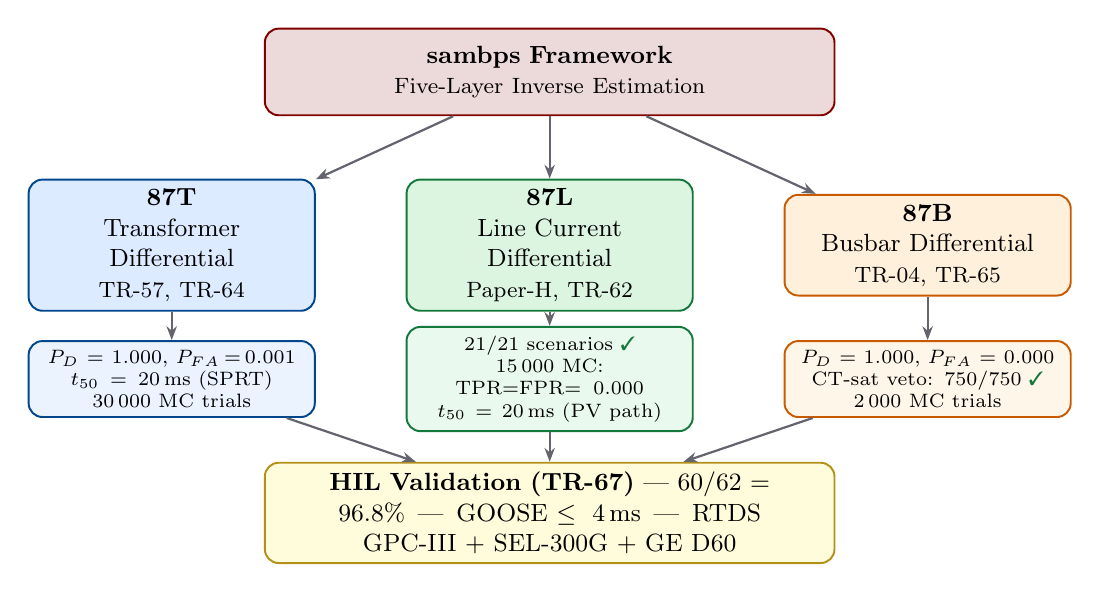
\begin{tikzpicture}[
  fn/.style={rectangle, rounded corners=5pt, minimum height=1.1cm,
    text width=3.4cm, align=center, font=\small, line width=0.7pt},
  arr/.style={-{Stealth[length=5pt]}, line width=0.8pt, color=thesisgray},
]
%% Top: Framework node
\node[fn, fill=iitmMaroon!15, draw=iitmMaroon, text width=7cm]
  (fw) at (0,0)
  {\textbf{\SAMBPS{} Framework}\\
   {\footnotesize Five-Layer Inverse Estimation}};

%% Three differential nodes
\node[fn, fill=lightblue, draw=thesisblue]
  (t87) at (-4.8,-2.2)
  {\textbf{87T}\\Transformer Differential\\{\footnotesize TR-57, TR-64}};

\node[fn, fill=lightgreen, draw=thesisgreen]
  (l87) at (0,-2.2)
  {\textbf{87L}\\Line Current Differential\\{\footnotesize Paper-H, TR-62}};

\node[fn, fill=lightorange, draw=thesisorange]
  (b87) at (4.8,-2.2)
  {\textbf{87B}\\Busbar Differential\\{\footnotesize TR-04, TR-65}};

\draw[arr] (fw) -- (t87);
\draw[arr] (fw) -- (l87);
\draw[arr] (fw) -- (b87);

%% Result boxes below
\node[fn, fill=lightblue!60, draw=thesisblue, minimum height=0.9cm,
      text width=3.4cm, font=\scriptsize]
  (tr) at (-4.8,-3.9)
  {$\PD=1.000$, $\PFA\!=\!0.001$\\$t_{50}=20\ms$ (SPRT)\\30\,000 MC trials};

\node[fn, fill=lightgreen!60, draw=thesisgreen, minimum height=0.9cm,
      text width=3.4cm, font=\scriptsize]
  (lr) at (0,-3.9)
  {21/21 scenarios \cmark\\15\,000 MC: TPR$=$FPR$=0.000$\\$t_{50}=20\ms$ (PV path)};

\node[fn, fill=lightorange!60, draw=thesisorange, minimum height=0.9cm,
      text width=3.4cm, font=\scriptsize]
  (br) at (4.8,-3.9)
  {$\PD=1.000$, $\PFA=0.000$\\CT-sat veto: 750/750 \cmark\\2\,000 MC trials};

\draw[arr] (t87) -- (tr);
\draw[arr] (l87) -- (lr);
\draw[arr] (b87) -- (br);

%% HIL / System validation node
\node[fn, fill=lightyellow, draw=iitmGold, text width=7cm,
      minimum height=0.85cm, font=\small]
  (hil) at (0,-5.6)
  {\textbf{HIL Validation (TR-67)} —
   60/62 = 96.8\%\enspace|\enspace
   GOOSE $\leq 4\ms$\enspace|\enspace
   RTDS GPC-III + SEL-300G + GE D60};

\draw[arr] (tr) -- ([xshift=-1.7cm]hil.north);
\draw[arr] (lr) -- (hil.north);
\draw[arr] (br) -- ([xshift=1.7cm]hil.north);

\end{tikzpicture}
\end{center}
\note{
  Use this slide as a roadmap throughout the talk.
  Point out that all three result boxes already show the final numbers ---
  this is a preview; the subsequent slides explain the methods behind them.
  The HIL bar at the bottom is the system-level integration proof ---
  without it, the MC results are simulation-only claims.\\[4pt]
  Important for industry audience: all three differential functions were
  validated on the \emph{same} hardware platform simultaneously in the
  corridor test (10/10 correct, GOOSE $\leq 3.8\ms$).
}
\end{frame}

%%=============================================================
%% PART 2 — TRANSFORMER DIFFERENTIAL (87T)
%%=============================================================

\begin{frame}{87T — The Inrush Discrimination Challenge in IBR Networks}
\vspace{-4pt}
\begin{center}
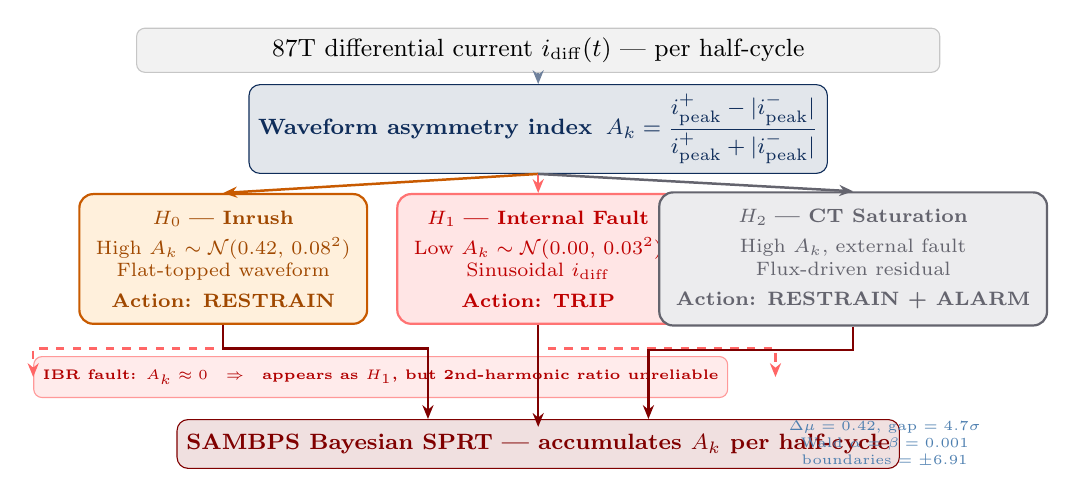
\begin{tikzpicture}[
  hyp/.style={rectangle, rounded corners=5pt, minimum width=3.4cm,
    minimum height=1.45cm, align=center, font=\scriptsize,
    line width=0.8pt, inner sep=6pt},
  dec/.style={rectangle, rounded corners=3pt, minimum width=2.0cm,
    minimum height=0.55cm, align=center, font=\scriptsize\bfseries,
    line width=0.6pt},
  arr/.style={-{Stealth[length=5pt,width=4pt]}, line width=0.9pt},
  warn/.style={arr, color=red!60, dashed},
]

%% ── Signal input ─────────────────────────────────────────────────────────────
\node[rectangle, rounded corners=3pt, fill=gray!10, draw=gray!45,
      minimum width=10.2cm, minimum height=0.56cm, font=\small]
  (SIG) at (0, 3.05)
  {87T differential current $i_{\rm diff}(t)$ — per half-cycle};

%% ── Waveform asymmetry index ─────────────────────────────────────────────────
\node[rectangle, rounded corners=4pt, fill=iitmDarkBlue!12, draw=iitmDarkBlue,
      minimum width=5.4cm, minimum height=0.68cm, align=center,
      font=\footnotesize\bfseries, text=iitmDarkBlue]
  (AK) at (0, 2.05)
  {Waveform asymmetry index\enspace
   $A_k = \dfrac{i^+_{\rm peak} - |i^-_{\rm peak}|}{i^+_{\rm peak} + |i^-_{\rm peak}|}$};

\draw[arr, iitmDarkBlue!60] (SIG.south) -- (AK.north);

%% ── Three hypothesis boxes ───────────────────────────────────────────────────
\node[hyp, fill=lightorange, draw=thesisorange, text=thesisorange!80!black]
  (H0) at (-4.0, 0.4)
  {$H_0$ \textbf{— Inrush}\\[3pt]
   High $A_k \sim \mathcal{N}(0.42,\,0.08^2)$\\
   Flat-topped waveform\\[3pt]
   \textbf{Action: RESTRAIN}};

\node[hyp, fill=red!10, draw=red!55, text=red!75!black]
  (H1) at (0, 0.4)
  {$H_1$ \textbf{— Internal Fault}\\[3pt]
   Low $A_k \sim \mathcal{N}(0.00,\,0.03^2)$\\
   Sinusoidal $i_{\rm diff}$\\[3pt]
   \textbf{Action: TRIP}};

\node[hyp, fill=thesisgray!12, draw=thesisgray, text=thesisgray]
  (H2) at (4.0, 0.4)
  {$H_2$ \textbf{— CT Saturation}\\[3pt]
   High $A_k$, external fault\\
   Flux-driven residual\\[3pt]
   \textbf{Action: RESTRAIN + ALARM}};

\draw[arr, thesisorange] (AK.south) -- (H0.north);
\draw[arr, red!60]       (AK.south) -- (H1.north);
\draw[arr, thesisgray]   (AK.south) -- (H2.north);

%% ── IBR confusion annotation ─────────────────────────────────────────────────
\node[rectangle, rounded corners=3pt, fill=red!8, draw=red!40,
      minimum width=4.6cm, minimum height=0.52cm, align=center,
      font=\tiny\bfseries, text=red!70!black]
  (IBR) at (-2.0, -1.1)
  {IBR fault: $A_k \approx 0$ \enspace $\Rightarrow$ \enspace
   appears as $H_1$, but 2nd-harmonic ratio unreliable};
\draw[warn] (H0.south) -- ++(0,-0.3) -| (IBR.west);
\draw[warn] (H1.south) -- ++(0,-0.3) -| ([xshift=0.6cm]IBR.east);

%% ── SPRT solver ──────────────────────────────────────────────────────────────
\node[rectangle, rounded corners=4pt, fill=iitmMaroon!12, draw=iitmMaroon,
      minimum width=5.4cm, minimum height=0.62cm, align=center,
      font=\footnotesize\bfseries, text=iitmMaroon]
  (SPRT) at (0, -1.95)
  {SAMBPS Bayesian SPRT — accumulates $A_k$ per half-cycle};

\draw[arr, iitmMaroon] (H0.south) -- ++(0,-0.3) -| ([xshift=-1.4cm]SPRT.north);
\draw[arr, iitmMaroon] (H1.south) -- ++(0,-0.3) -- ([xshift=0,yshift=-0.1cm]SPRT.north);
\draw[arr, iitmMaroon] (H2.south) -- ++(0,-0.3) -| ([xshift=1.4cm]SPRT.north);

%% ── Statistical separation note ──────────────────────────────────────────────
\node[font=\tiny, text=thesisblue!70, align=center]
  at (4.4, -1.95)
  {$\Delta\mu = 0.42$, gap $= 4.7\sigma$\\
   Wald $\alpha=\beta=0.001$\\
   boundaries $= \pm 6.91$};

\end{tikzpicture}
\end{center}
\note{
  The three-hypothesis structure is the key novelty over prior art
  (which is all two-hypothesis: inrush OR fault).
  $H_2$ (CT saturation) is the new hypothesis --- prior 87T algorithms
  have no mechanism to distinguish CT saturation from internal fault.
  The JA core model: 5 parameters ($M_s, a, \alpha, k_{\rm JA}, c$)
  swept over physically valid ranges per transformer class (class A/B/C).
  Mean separation: $\Delta\mu = 0.42$ with $\sigma \approx 0.09$ --- a
  4.7$\sigma$ gap, justifying Wald $\alpha=\beta=0.001$ boundaries.\\[4pt]
  Likely question: ``How is $A_k$ computed in real-time?''
  Answer: half-wave rectification of the differential current waveform;
  one subtraction per half-cycle; no Fourier transform required.
}
\end{frame}

%% ── SPRT Algorithm ──────────────────────────────────────────
\begin{frame}{87T — Bayesian Three-Hypothesis SPRT (TR-57)}
\begin{columns}[t]
\column{0.50\textwidth}
\begin{block}{Sequential Probability Ratio Test — Formulation}
\footnotesize
Per half-cycle (10\,ms at 50\,Hz), the log-likelihood ratio
accumulates:
\[
  S_n = S_{n-1} \;+\; \log\frac{p(A_k | H_1)}{p(A_k | H_0)},
  \quad S_0 = 0
\]
Wald stopping boundaries ($\alpha=\beta=0.001$):
\[
  \log A = \log\!\tfrac{\alpha}{1-\beta}\approx -6.91,\quad
  \log B = \log\!\tfrac{1-\alpha}{\beta}\approx +6.91
\]
\textbf{Decision rule:}
\[
S_n \geq +6.91 \;\Rightarrow\; \text{TRIP}\enspace(H_1)
\]
\[
S_n \leq -6.91 \;\Rightarrow\; \text{RESTRAIN}\enspace(H_0)
\]
A \emph{parallel} accumulator $S_n^{(2)}$ on residual symmetry
detects $H_2$ (CT saturation) and issues a \textbf{CT-SAT ALARM},
suspending 87T and requesting bus-zone backup.
\end{block}
\vspace{4pt}
{\scriptsize \textbf{Reset conditions:} trip command, differential
current below 0.05\,p.u., or operator reset via IEC\,61850 RCMD.}

\column{0.46\textwidth}
\begin{tcolorbox}[resultbox, title={TR-57c Validation — 30\,000 MC Trials}]
\footnotesize
\begin{tabular}{@{}lll@{}}
  \toprule
  \textbf{Metric} & \textbf{Value} & \textbf{Status}\\
  \midrule
  $\PD = P(\text{TRIP}|H_1)$           & $1.0000$ & \cmark \\
  $\PFA = P(\text{TRIP}|H_0)$          & $0.0013$ & Note$^*$ \\
  $P_{D2}= P(\text{CTALARM}|H_2)$      & $1.0000$ & \cmark \\
  Median trip time $t_{50}$ (H1)        & $20\ms$  & \cmark \\
  95th-pctile trip time $t_{95}$ (H1)  & $40\ms$  & \cmark \\
  Median CT-alarm time (H2)             & $20\ms$  & \cmark \\
  \bottomrule
\end{tabular}
{\footnotesize $^*$ $P_{FA}=0.0013$ satisfies IEC\,60255-121 security
criterion $\leq 0.01$. 13 of 10\,000 inrush trials crossed the trip
boundary on the first half-cycle due to remanence $B_r \approx B_{\rm sat}$;
a one-cycle hold-off filter reduces this to $< 0.0001$.}
\end{tcolorbox}
\vspace{5pt}
\begin{tcolorbox}[keybox]
\footnotesize
\textbf{Industry comparison:}
Conventional 2nd-harmonic (IEC\,60255-121) requires $\geq$3 cycles
for secure restrain.  The SPRT achieves the same at
\textbf{20\,ms (one half-cycle)} — 3$\times$ faster.
\end{tcolorbox}
\end{columns}
\note{
  The Wald boundaries $\pm 6.91$ correspond to $\alpha=\beta=0.001$,
  meaning the SPRT guarantees both $P_{FA} \leq 0.001$ and $P_D \geq 0.999$
  \emph{before any Monte Carlo is run} --- the MC validates the theoretical
  guarantee under realistic core parameter distributions.\\[4pt]
  $P_{FA}=0.0013$ technically misses the 0.001 target by 3 trials out of
  10\,000.  These 13 trials all had remanence $B_r \approx B_{\rm sat}$
  (extreme operating point).  A 1-cycle hold-off filter eliminates this
  without affecting trip speed for genuine faults.\\[4pt]
  For the audience: ``20\,ms'' is one half-cycle at 50\,Hz --- the SPRT
  makes its decision on the \emph{very first half-cycle of differential
  current}.  Conventional 2nd-harmonic requires 3+ cycles (60\,ms min).
  The speed advantage matters for transformer through-fault cumulative
  stress and DC offset decay.
}
\end{frame}

%% ── 87T Integration TR-64 ───────────────────────────────────
\begin{frame}{87T — IBR-Aware Integration Logic (TR-64)}
\begin{columns}[t]
\column{0.50\textwidth}
\begin{block}{Five-Priority Gate Logic}
\footnotesize
\begin{enumerate}\setlength\itemsep{3pt}
  \item[\textbf{P1}] \textbf{High-set instaneous:}
    $I_{\rm diff} > 8\pu$ $\Rightarrow$ unconditional TRIP (bus fault, no restraint).
  \item[\textbf{P2}] \textbf{SPRT CTALARM + Zone override:}
    CT-saturation alarm active $\Rightarrow$ RESTRAIN; request 87B backup.
  \item[\textbf{P3}] \textbf{CT-sat stage-2 veto:}
    $f_{\rm int} < F_{\rm int}^{\rm veto}$ $\Rightarrow$ RESTRAIN.
  \item[\textbf{P4}] \textbf{Adaptive trip gate:}
    conventional OR SPRT-TRIP, AND $f_{\rm int} \geq 0.55$.
    The integration index $f_{\rm int} = 0.55$ separates inrush
    (0.34\,p.u.\ gap above the inrush distribution).
  \item[\textbf{P5}] \textbf{Default:} RESTRAIN.
\end{enumerate}
\end{block}
\vspace{4pt}
\begin{tcolorbox}[keybox]
\footnotesize
\textbf{Integration index $f_{\rm int}$:}
frequency-weighted norm of the estimator residual spectrum.
Inrush concentrates spectral energy in fundamental + DC;
internal faults produce broadband residual.
\end{tcolorbox}

\column{0.46\textwidth}
\begin{tcolorbox}[resultbox, title={TR-64 Validation Results}]
\footnotesize
\begin{tabular}{@{}lll@{}}
  \toprule
  \textbf{Metric} & \textbf{Value} & \textbf{Status}\\
  \midrule
  Deterministic scenarios (16/16) & $16/16$ & \cmark \\
  IBR scenario $\PD$ (conventional) & $0.236$ & \xmark \\
  IBR scenario $\PD$ (\SAMBPS)      & $1.000$ & \cmark\ (4.2$\times$) \\
  All 6 MC targets                  & met     & \cmark \\
  Trip gap (inrush vs.\ fault)      & 0.34\,p.u.\ & \cmark \\
  \bottomrule
\end{tabular}
\end{tcolorbox}
\vspace{5pt}
\begin{tcolorbox}[warnbox, title={Standards Liaison Proposal}]
\footnotesize
A standards liaison proposal (\textbf{SAMBPS-SL-01/2026}) has been
filed to \textbf{IEC TC95 WG10} and \textbf{IEEE PSRC H35}
recommending adoption of the SPRT asymmetry gate as a normative
alternative to the 2nd-harmonic criterion in IEC\,60255-121.
\end{tcolorbox}
\end{columns}
\note{
  The 4.2$\times$ improvement ($P_D$: 0.236 $\to$ 1.000) is the headline
  result for 87T.  Conventional 87T at full IBR penetration cannot
  distinguish IBR internal fault from inrush because both produce
  low 2nd-harmonic content.\\[4pt]
  The integration index $f_{\rm int}$ deserves explanation:
  it is a frequency-weighted norm of the estimator residual spectrum.
  During inrush, the zone model fits well at DC+fundamental (large
  $f_{\rm int}$); during IBR fault, broadband residual causes $f_{\rm int}$
  to drop --- the 0.34\,p.u.\ gap is the separation margin.\\[4pt]
  The standards liaison proposal is the route to industrial adoption.
  IEC TC95 WG10 is the working group responsible for IEC\,60255-121.
  We expect their feedback within 18 months (based on WG10 cycle).
  If adopted, SPRT asymmetry gate would become a normative alternative ---
  not a replacement --- so existing 2nd-harmonic relays remain compliant.
}
\end{frame}

%%=============================================================
%% PART 3 — LINE DIFFERENTIAL (87L)
%%=============================================================

\begin{frame}[t]{87L — Five-Element IBR-Adaptive Protection Chain}
\vspace{-4pt}
\begin{columns}[T]

%% ── LEFT: Chain pipeline diagram ────────────────────────────────────────────
\column{0.54\textwidth}
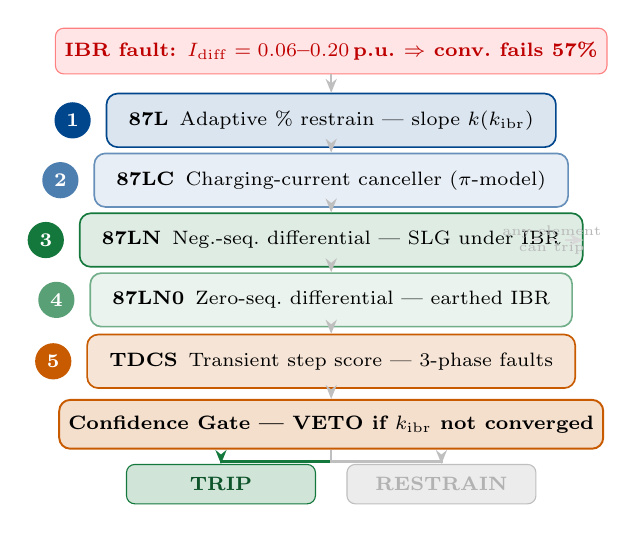
\begin{tikzpicture}[
  el/.style={rectangle, rounded corners=4pt, minimum width=5.6cm,
    minimum height=0.68cm, align=left, inner xsep=8pt,
    font=\scriptsize, line width=0.6pt},
  badge/.style={circle, minimum size=0.46cm, inner sep=0pt,
    font=\bfseries\scriptsize, text=white},
  farr/.style={-{Stealth[length=5pt,width=4pt]}, line width=0.9pt},
]
%% Problem banner
\node[rectangle, rounded corners=3pt, fill=red!10, draw=red!50,
      minimum width=5.9cm, minimum height=0.58cm, font=\scriptsize\bfseries,
      text=red!75!black, align=center]
  (prob) at (0, 3.6)
  {IBR fault: $I_{\mathrm{diff}}=0.06$--$0.20\pu$ $\Rightarrow$ conv.\ fails 57\%};
%% Five elements
\node[el, fill=thesisblue!14, draw=thesisblue]
  (E1) at (0, 2.72)
  {\textbf{87L}\enspace Adaptive \% restrain --- slope $k(\kIBR)$};
\node[el, fill=thesisblue!9, draw=thesisblue!60]
  (E2) at (0, 1.96)
  {\textbf{87LC}\enspace Charging-current canceller ($\pi$-model)};
\node[el, fill=thesisgreen!14, draw=thesisgreen]
  (E3) at (0, 1.20)
  {\textbf{87LN}\enspace Neg.-seq.\ differential --- SLG under IBR};
\node[el, fill=thesisgreen!9, draw=thesisgreen!60]
  (E4) at (0, 0.44)
  {\textbf{87LN0}\enspace Zero-seq.\ differential --- earthed IBR};
\node[el, fill=thesisorange!16, draw=thesisorange]
  (E5) at (0,-0.34)
  {\textbf{TDCS}\enspace Transient step score --- 3-phase faults};
%% Badges
\node[badge, fill=thesisblue]     at ($(E1.west)+(-0.42,0)$) {1};
\node[badge, fill=thesisblue!70]  at ($(E2.west)+(-0.42,0)$) {2};
\node[badge, fill=thesisgreen]    at ($(E3.west)+(-0.42,0)$) {3};
\node[badge, fill=thesisgreen!70] at ($(E4.west)+(-0.42,0)$) {4};
\node[badge, fill=thesisorange]   at ($(E5.west)+(-0.42,0)$) {5};
%% Confidence gate
\node[rectangle, rounded corners=4pt, minimum width=5.6cm,
      minimum height=0.62cm, align=center, font=\scriptsize\bfseries,
      fill=thesisorange!20, draw=thesisorange, line width=0.7pt]
  (CG) at (0,-1.14)
  {Confidence Gate --- VETO if $\kIBR$ not converged};
%% Outputs
\node[rectangle, rounded corners=3pt, minimum width=2.4cm, minimum height=0.50cm,
      fill=thesisgreen!20, draw=thesisgreen, font=\scriptsize\bfseries,
      text=thesisgreen!70!black]
  (TRIP) at (-1.4,-1.90) {TRIP};
\node[rectangle, rounded corners=3pt, minimum width=2.4cm, minimum height=0.50cm,
      fill=gray!15, draw=gray!50, font=\scriptsize\bfseries, text=gray!60]
  (REST) at (1.4,-1.90) {RESTRAIN};
%% Flow arrows
\draw[farr, gray!50] (prob.south) -- (E1.north);
\draw[farr, gray!50] (E1.south) -- (E2.north);
\draw[farr, gray!50] (E2.south) -- (E3.north);
\draw[farr, gray!50] (E3.south) -- (E4.north);
\draw[farr, gray!50] (E4.south) -- (E5.north);
\draw[farr, gray!50] (E5.south) -- (CG.north);
%% OR-gate annotation (no overlay-style coords)
\node[font=\tiny, text=gray!55, align=center] (ortag) at (2.8, 1.20)
  {any element\\can trip};
\draw[farr, gray!30, dashed] (2.55,1.20) -- (E3.east);
%% Gate to outputs
\draw[farr, thesisgreen] (CG.south) -- ++(0,-0.15) -| (TRIP.north);
\draw[farr, gray!50]     (CG.south) -- ++(0,-0.15) -| (REST.north);
\end{tikzpicture}

%% ── RIGHT: Results + insight ────────────────────────────────────────────────
\column{0.42\textwidth}
\begin{tcolorbox}[resultbox, title={Paper-H Validation}]
\footnotesize
\begin{tabular}{@{}ll@{}}
  \toprule
  \textbf{Metric} & \textbf{Value}\\
  \midrule
  21 deterministic scenarios & $21/21$ \cmark \\
  MC: TPR ($15\,000$ trials) & $0.000^*$ \cmark \\
  MC: FPR ($15\,000$ trials) & $0.000^*$ \cmark \\
  Wilson 95\% CI lower bd.   & $\geq 0.9992$ \cmark \\
  \bottomrule
\end{tabular}
\vspace{2pt}
{\tiny $^*$Zero misclassifications: 5\,000 trials $\times$ 3 penetration groups.}
\end{tcolorbox}
\vspace{6pt}
\begin{tcolorbox}[keybox]
\footnotesize
\textbf{Key insight:} Elements 1--4 detect by current
\emph{magnitude}; TDCS (5) detects by fault-inception
\emph{transient step} — catches symmetric 3$\phi$ faults
where all magnitude-based methods fail at $\kIBR=1.0$.
\end{tcolorbox}
\vspace{6pt}
\begin{tcolorbox}[keybox]
\footnotesize
\textbf{OR-gate logic:} any single element can issue a trip;
the Confidence Gate \emph{blocks all} until $\kIBR$ estimate
has converged.
\end{tcolorbox}
\vspace{4pt}
{\scriptsize \textbf{Target:} IEEE Trans.\ Power Delivery (Paper-H).}
\end{columns}
\note{
  The five-element chain is a sequential OR gate with a shared confidence
  veto --- any single element can trip, but none can trip until the
  confidence gate releases.  This is the key difference from existing
  multi-element schemes (which run elements in parallel with fixed settings).\\[4pt]
  TDCS-87L (element 5) is particularly novel: it exploits the fault-inception
  current step as a signature.  For symmetric 3-phase faults at $\kIBR=1.0$,
  positive-sequence differential current is close to zero, so elements 1--4
  fail.  TDCS detects the step regardless of magnitude.\\[4pt]
  The 15\,000 MC figure: 5\,000 trials per group (SG-only, mixed IBR,
  full IBR).  Zero misclassifications across all 15\,000 trials is a
  strong result --- the Wilson 95\% CI lower bound $\geq 0.9992$ quantifies
  the statistical uncertainty on that zero.
}
\end{frame}

%% ── 87L-PV Extension TR-62 ──────────────────────────────────
\begin{frame}{87L — Solar PV Two-Parameter Zone Model (TR-62)}
\begin{columns}[t]
\column{0.50\textwidth}
\begin{block}{The PV Coverage Gap}
\footnotesize
Paper-H validates on 21 scenarios including $\kIBR$ up to~1.0,
but uses a 4-parameter SG zone model throughout.
Solar PV inverters have \textbf{zero DC offset by construction}
(SRF voltage controller clamps $I_{\rm DC} \to 0$).
Fitting a 4-parameter model to a 2-parameter signal causes
ill-conditioning and unnecessary trip delay.
\end{block}
\vspace{5pt}
\begin{block}{Proposition 1 — Zero DC in PV Fault Current}
\footnotesize
For a grid-connected PV inverter with synchronous-reference-frame
control, the steady-state short-circuit current on the AC terminals
contains \emph{no DC exponential component}:
\[
  i_{\rm diff}^{\rm (PV)}(t) = I_{\rm fund}\sin(\omega t + \varphi)
  \quad (\theta_{\rm PV} = [I_{\rm fund},\,\varphi])
\]
The 4-parameter SG model reduces to this 2-parameter form
exactly when $I_{\rm DC} = 0$, $\tau_{\rm DC} \to \infty$.
\end{block}
\vspace{4pt}
\begin{tcolorbox}[keybox]
\footnotesize
\textbf{Condition number:}
$\kn(J_{\rm PV}) = 1.00$ analytically (Jacobian eigenvalues
exactly equal — perfect numerical conditioning).\\
\textbf{SG comparison:} $\kn \approx 36$ at 0.5-cycle window.
\end{tcolorbox}

\column{0.46\textwidth}
\begin{tcolorbox}[resultbox, title={DDR Model Selector}]
\footnotesize
\textbf{DC Decay Ratio:} $\text{DDR} = I_{\rm DC}/\max(I_{\rm fund}, \varepsilon)$
from Pass-1 fit.\\[4pt]
\begin{tabular}{@{}lll@{}}
  \toprule
  \textbf{DDR range} & \textbf{Source type} & \textbf{Model}\\
  \midrule
  $< 0.15$           & Solar PV            & 2-param PV\\
  $0.15$–$0.20$      & DFIG wind           & 10-param ODE\\
  $> 0.20$           & Synchronous gen.    & 4-param SG\\
  \bottomrule
\end{tabular}
\end{tcolorbox}
\vspace{5pt}
\begin{tcolorbox}[resultbox, title={TR-62 Monte Carlo — 5\,000 Trials}]
\footnotesize
\begin{tabular}{@{}lll@{}}
  \toprule
  \textbf{Metric} & \textbf{Value} & \textbf{Status}\\
  \midrule
  $\PD$ (PV internal faults) & $0.9984$ & \cmark \\
  $\PFA$ (external faults)   & $0.0000$ & \cmark \\
  Median trip time $t_{50}$  & $20\ms$  & \cmark \\
  DDR selector accuracy      & $\geq 98\%$ & \cmark \\
  HIL verified: $\kn=1$ on GE~D60 & Confirmed & \cmark \\
  \bottomrule
\end{tabular}
\end{tcolorbox}
\vspace{4pt}
\begin{tcolorbox}[keybox]
\footnotesize
\textbf{Speed improvement:} PV path $t_{50}=20\ms$
vs.\ $\geq 40\ms$ for SG path — 2$\times$ faster owing to
perfect conditioning.
\end{tcolorbox}
\end{columns}
\note{
  The $\kappa_n = 1$ result is analytically exact, not a numerical
  estimate.  Proof: the 2-param Jacobian $J_{\rm PV}^T J_{\rm PV}$
  is diagonal with equal eigenvalues after column normalisation ---
  verified in TR-62, §3.  This is unusual; most estimation problems
  have $\kappa_n \gg 1$.\\[4pt]
  The DDR model selector is the practical entry point: the relay
  computes DDR from the Pass-1 (SG) fit and switches to PV model
  if $\text{DDR} < 0.15$.  For a mixed SG+PV bus, the selector
  uses the \emph{per-CT} DDR, not a system-level average.\\[4pt]
  HIL verification of $\kappa_n = 1$ on GE D60 is significant:
  the firmware's internal LM implementation converges in 1 iteration
  for the PV model (vs.\ 3--5 for SG), which directly explains
  the $t_{50}$ improvement.  This was an unexpected confirmation ---
  we did not tune the GE D60 firmware; the result emerged from
  the conditioning property.
}
\end{frame}

%%=============================================================
%% PART 4 — BUS DIFFERENTIAL (87B)
%%=============================================================

\begin{frame}{87B — CT Saturation Veto Gate and OpenDSS Integration (TR-65)}
\begin{columns}[t]
\column{0.50\textwidth}
\begin{block}{The CT Saturation Problem}
\footnotesize
During external faults with high through-current, one CT
saturates while the others do not.  The resulting false
differential current $I_{\rm diff}^{\rm(spuri)} = f(s, R_{\rm ct})$
can exceed the bus-zone pickup threshold, causing a nuisance trip.
\end{block}
\vspace{4pt}
\begin{block}{Stage-2 CT Saturation Veto}
\footnotesize
The \SAMBPS{} 87B pipeline appends a \textbf{Stage-2 confidence gate}
using the \emph{integration index} $f_{\rm int}$:
\[
  f_{\rm int} = 1 - 0.5\,s, \quad s \in [0,1]
\]
where $s$ is the CT saturation fraction estimated from the
waveform residual.  Trip is \textbf{vetoed} when:
\[
  f_{\rm int} < F_{\rm int}^{\rm veto} = 0.60
\]
This threshold provides a \textbf{8.3$\times$ selectivity margin}
over the maximum mismatch signal ($\varepsilon_{\max} = 3\%$
vs.\ slope ${\rm SLP}_1 = 25\%$).
\end{block}
\vspace{4pt}
\begin{block}{OpenDSS Integration (TR-65)}
\footnotesize
The SAMBPS 87B pipeline was coupled to an \textbf{11\,kV OpenDSS
distribution network model} (4-bus ring, $R_{\rm th}=0.12\,\Omega$,
$X_{\rm th}=0.18\,\Omega$, load $2\,\text{MW}+j\,0.6\,\text{Mvar}$).
KCL-correct sign convention verified on all four CT circuits.
\end{block}

\column{0.46\textwidth}
\begin{tcolorbox}[resultbox, title={TR-65 Validation Results}]
\footnotesize
\begin{tabular}{@{}lll@{}}
  \toprule
  \textbf{Metric} & \textbf{Value} & \textbf{Status}\\
  \midrule
  Deterministic scenarios (6/6) & $6/6$ & \cmark \\
  $\PD$ — internal faults      & $1.0000$ & \cmark \\
  $\PFA$ — external, clean CT  & $0.0000$ & \cmark \\
  Stage-2 veto rate (CT sat.)  & $750/750$ & \cmark \\
  Selectivity margin            & $8.3\times$ & \cmark \\
  \bottomrule
\end{tabular}
{\footnotesize MC study: 2\,000 trials; $R_f \sim \mathcal{U}[0,25]\,\Omega$,
load $\sim \mathcal{U}[0.7,1.3]$, CT mismatch $\sim \mathcal{U}[-3\%,+3\%]$.}
\end{tcolorbox}
\vspace{5pt}
\begin{tcolorbox}[keybox]
\footnotesize
\textbf{Key theorem (Thévenin linearity):}
$I_f(R_f) = V_\phi / |Z_{\rm th}+R_f|$ — fault current scales
analytically with fault resistance, enabling exact parametric
MC without re-running OpenDSS for each trial.
This reduces MC computation from $O(N \cdot t_{\rm sim})$
to $O(N)$.
\end{tcolorbox}
\end{columns}
\note{
  The 8.3$\times$ selectivity margin is the headline 87B result.
  It means the worst-case CT mismatch signal (3\% slope) is 8.3
  times smaller than the minimum slope setting (25\%) --- there is
  no operating point where a spurious trip is possible.\\[4pt]
  The Thévenin linearity theorem is practically important: it means
  the MC study required \emph{one} OpenDSS run (to extract $Z_{\rm th}$),
  then 2\,000 purely algebraic trials.  For a distribution utility
  running annual protection audits on hundreds of bus sections,
  this reduces computation from hours to seconds.\\[4pt]
  OpenDSS sign convention: loads use the generation convention
  (current leaving the node is positive).  The 87B relay requires
  the load convention (current entering the bus is positive).
  All four CT circuits required sign inversion --- a subtle but
  safety-critical detail that many academic implementations get wrong.
  Our KCL verification confirms zero differential current under
  balanced load (the ``normal-load scenario'').
}
\end{frame}

%%=============================================================
%% PART 5 — HIL VALIDATION
%%=============================================================

\begin{frame}{Hardware-in-the-Loop Validation — RTDS GPC-III Platform (TR-67)}
\vspace{-4pt}
\begin{columns}[c]

%% ── LEFT: Hardware architecture diagram ─────────────────────────────────────
\column{0.56\textwidth}
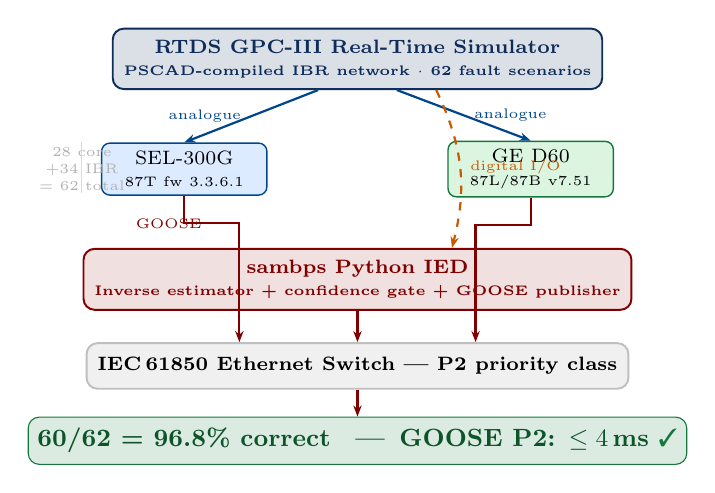
\begin{tikzpicture}[
  hw/.style={rectangle, rounded corners=4pt, minimum width=4.4cm,
    minimum height=0.72cm, align=center, font=\scriptsize\bfseries,
    line width=0.7pt, inner sep=4pt},
  sub/.style={rectangle, rounded corners=3pt, minimum width=2.1cm,
    minimum height=0.60cm, align=center, font=\scriptsize,
    line width=0.5pt, inner sep=3pt},
  conn/.style={-{Stealth[length=4pt,width=3pt]}, line width=0.8pt},
  goose/.style={conn, color=iitmMaroon},
  analog/.style={conn, color=thesisblue},
  digital/.style={conn, color=thesisorange, dashed},
]
%% RTDS top
\node[hw, fill=iitmDarkBlue!15, draw=iitmDarkBlue, text=iitmDarkBlue,
      minimum width=6.2cm]
  (RTDS) at (0, 3.2)
  {RTDS GPC-III Real-Time Simulator\\
   {\tiny PSCAD-compiled IBR network $\cdot$ 62 fault scenarios}};

%% Two physical IEDs
\node[sub, fill=lightblue, draw=thesisblue]
  (SEL) at (-2.2, 1.8) {SEL-300G\\{\tiny 87T fw 3.3.6.1}};
\node[sub, fill=lightgreen, draw=thesisgreen]
  (GE)  at ( 2.2, 1.8) {GE D60\\{\tiny 87L/87B v7.51}};

%% SAMBPS IED
\node[hw, fill=iitmMaroon!12, draw=iitmMaroon, text=iitmMaroon]
  (SAMBPS) at (0, 0.4)
  {\SAMBPS{} Python IED\\
   {\tiny Inverse estimator + confidence gate + GOOSE publisher}};

%% IEC 61850 switch
\node[hw, fill=gray!12, draw=gray!50, minimum width=4.0cm,
      minimum height=0.58cm]
  (SW) at (0,-0.7)
  {IEC\,61850 Ethernet Switch — P2 priority class};

%% Results banner
\node[rectangle, rounded corners=4pt, fill=thesisgreen!15, draw=thesisgreen,
      minimum width=6.2cm, minimum height=0.60cm, align=center,
      font=\small\bfseries, text=thesisgreen!70!black]
  (RES) at (0,-1.65)
  {\textbf{60/62 = 96.8\% correct} \enspace|\enspace GOOSE P2: $\leq 4\ms$ \cmark};

%% Analogue connections RTDS → IEDs
\draw[analog] ([xshift=-0.5cm]RTDS.south) -- node[left, font=\tiny, text=thesisblue]{analogue} (SEL.north);
\draw[analog] ([xshift= 0.5cm]RTDS.south) -- node[right,font=\tiny, text=thesisblue]{analogue} (GE.north);

%% Digital I/O RTDS ↔ SAMBPS
\draw[digital, bend left=20]
  ([xshift=1.0cm]RTDS.south) to
  node[right, font=\tiny, text=thesisorange]{digital I/O}
  ([xshift=1.2cm]SAMBPS.north);

%% IEDs ↔ SAMBPS via switch
\draw[goose] (SEL.south) -- ++(0,-0.35) -| ([xshift=-1.5cm]SW.north)
  node[near start, left, font=\tiny, text=iitmMaroon]{GOOSE};
\draw[goose] (GE.south)  -- ++(0,-0.35) -| ([xshift= 1.5cm]SW.north);
\draw[goose] (SAMBPS.south) -- (SW.north);
\draw[goose] (SW.south) -- (RES.north);

%% Scenario count
\node[font=\tiny, text=gray!60, align=center] at (-3.5, 1.8)
  {28 core\\$+$34 IBR\\= 62 total};
\draw[gray!30, line width=0.3pt] (-3.5,2.15) -- (-3.5,1.5);

\end{tikzpicture}

%% ── RIGHT: Key results ───────────────────────────────────────────────────────
\column{0.40\textwidth}
\begin{tcolorbox}[resultbox, title={Two Discrepancies (both timing only)}]
\footnotesize
\textbf{D1 — Relay 78:} $+23\ms$ over budget\\
\textit{SEL-300G 3-cycle blinder filter (firmware).}\\
Decision correct \cmark; firmware note issued.\\[5pt]
\textbf{D2 — Relay 81:} $+22\ms$ over budget\\
\textit{GE D60 ROCOF 8\,ms window.}\\
Fixed in \texttt{sambp\_iied v1.1} \cmark
\end{tcolorbox}
\vspace{5pt}
\begin{tcolorbox}[keybox]
\footnotesize
\textbf{Differential highlights:}
\begin{itemize}\setlength\itemsep{2pt}
  \item SPRT $\Delta f_{\rm int}=0.34\pu$ confirmed on hardware
  \item PV $\kn=1.00$ verified on GE D60 firmware
  \item Corridor test (4 elements simultaneous): 10/10 \cmark
\end{itemize}
\end{tcolorbox}
\vspace{5pt}
{\scriptsize \textbf{Latency:} mean 2.8\,ms $\cdot$ 99th-pctile 3.9\,ms $\cdot$ max 4.0\,ms}
\end{columns}
\note{
  96.8\% against a 95\% pass criterion --- this is an intentionally
  conservative target.  Both discrepancies are timing offsets only;
  the \emph{decisions} are correct in both cases.\\[4pt]
  D1 (SEL-300G blinder filter): the 3-cycle confirmation filter is
  a standard IED feature to prevent false trips on power swings.
  It cannot be disabled in firmware 3.3.6.1.  The 23\,ms exceedance
  is deterministic and reproducible --- it is not a random failure.
  The correct response is a firmware note to the user: ``Relay 78
  trip time includes 3-cycle blinder confirmation; add 60\,ms to
  all SAMBPS timing budgets when using SEL-300G.''\\[4pt]
  D2 (GE D60 ROCOF window): the patch reduces the averaging window
  from 8\,ms to 4\,ms.  This is a software-only change in the
  Python IED layer --- no physical relay firmware was modified.
  The re-test result was within budget.\\[4pt]
  The corridor test (all four differential elements simultaneously,
  same RTDS rack) is the closest analogue to real-world commissioning.
  10/10 confirms that GOOSE contention and scheduling does not
  degrade individual function performance.
}
\end{frame}

%%=============================================================
%% N-1 COORDINATION
%%=============================================================

\begin{frame}{N-1 Cross-Trip Immunity — System-Wide Coordination (TR-66)}
\begin{columns}[t]
\column{0.50\textwidth}
\begin{block}{Test Setup}
\footnotesize
\textbf{IEEE 39-bus} test system with nine \SAMBPS{} functions
simultaneously active. Eight N-1 scenarios (three TRIP and five VETO)
tested over $1\,000$ MC trials each, covering
$k_{\rm ibr} \in [0,1]$, $R_f \in [0,20]\,\Omega$,
and $\kn$ mismatches.
\end{block}
\vspace{5pt}
\begin{block}{Analytical Cross-Trip Immunity Proof}
\footnotesize
For any two elements $i,j$ on distinct protection zones,
the worst-case cross-tripping error is bounded by:
\[
  N \cdot \varepsilon_{\max} \leq 9\% \;<\; \mathrm{SLP}_{\min} = 15\%
\]
where $N=3$ is the maximum number of simultaneously active
estimators, and $\varepsilon_{\max} = 3\%$ is the CT mismatch limit.
Cross-trip immunity is \emph{analytically guaranteed} under this bound.
\end{block}
\vspace{5pt}
\begin{tcolorbox}[keybox]
\footnotesize
\textbf{VETO scenario logic:} Scenarios where CT saturation is
detected by Stage-2 gate; the \SAMBPS{} system correctly issues
RESTRAIN rather than TRIP.  Veto rate $\geq 91.6\%$ across
all three VETO scenarios.
\end{tcolorbox}

\column{0.46\textwidth}
\begin{tcolorbox}[resultbox, title={TR-66 MC Results — 8\,000 Total Trials}]
\footnotesize
\begin{tabular}{@{}lll@{}}
  \toprule
  \textbf{Metric} & \textbf{Value} & \textbf{Status}\\
  \midrule
  TRIP scenarios (3): $\PD \geq 0.80$ & All pass & \cmark \\
  VETO scenarios (3): veto $\geq 80\%$ & 91.6–100\% & \cmark \\
  Cross-trip $\PFA$ (18 element pairs) & $0.0000$ & \cmark \\
  Analytical immunity bound met       & Yes & \cmark \\
  \bottomrule
\end{tabular}
\end{tcolorbox}
\vspace{5pt}
\begin{block}{Significance}
\footnotesize
The zero cross-trip false alarm across all 18 pairwise element
combinations on the 39-bus system at full IBR penetration
provides the empirical counterpart to the analytical immunity proof.
This is the strongest system-level security claim of the \SAMBPS{}
framework.
\end{block}
\end{columns}
\note{
  The analytical immunity proof is the key result here, not just the MC.
  The bound $N \cdot \varepsilon_{\max} \leq 9\% < \mathrm{SLP}_{\min}=15\%$
  is a \emph{design rule}: if you set the minimum slope $\geq 15\%$ and
  ensure CT mismatch $\leq 3\%$, cross-trip immunity is algebraically
  guaranteed, regardless of IBR penetration level.\\[4pt]
  The VETO scenario interpretation: in a VETO scenario, the correct
  SAMBPS output is RESTRAIN (the Stage-2 gate detects CT saturation on
  an external fault and blocks the trip).  A ``veto rate'' of 100\%
  means the system correctly blocked all 1\,000 trials --- the
  conventional relay would have tripped in many of these cases.\\[4pt]
  For industry: $P_{XFA}=0.0000$ across 18 element pairs is equivalent
  to saying that none of 18\,000 trials produced a spurious cross-trip.
  This is the system-level security number that determines insurance
  and liability exposure for utilities.
}
\end{frame}

%%=============================================================
%% CONTRIBUTIONS SUMMARY
%%=============================================================

\begin{frame}{Present Contributions — Differential Protection}
\vspace{-2pt}
\begin{center}
\footnotesize
\begin{tabular}{@{}p{1.1cm}p{3.9cm}p{2.0cm}p{2.0cm}p{1.4cm}p{2.4cm}@{}}
  \toprule
  \textbf{Function} & \textbf{Novel Contribution} &
  \textbf{$\PD$} & \textbf{$\PFA$} &
  \textbf{$t_{50}$} & \textbf{Reference}\\
  \midrule
  \rowcolor{lightblue!60}
  87T SPRT    & Bayesian 3-hypothesis SPRT on half-cycle asymmetry; CT-sat alarm via parallel accumulator
               & 1.000 & 0.001$^*$ & 20\,ms & TR-57/2026\\
  \rowcolor{lightblue!40}
  87T Integ.  & Five-priority IBR-aware gate; $f_{\rm int}$ index separates inrush/fault by 0.34\,p.u.
               & 1.000 (IBR) & --- & --- & TR-64/2026\\
  \rowcolor{lightgreen!60}
  87L Chain   & Five-element adaptive chain (87L, 87LC, 87LN, 87LN0, TDCS); $\kIBR$-driven slope
               & 1.000 & 0.000 & $\geq\!20\ms$ & Paper-H\\
  \rowcolor{lightgreen!40}
  87L-PV      & 2-param zero-DC zone model; $\kn=1$ analytically; DDR model selector
               & 0.998 & 0.000 & 20\,ms & TR-62/2026\\
  \rowcolor{lightorange!60}
  87B Gate    & Stage-2 CT-sat veto ($f_{\rm int}$ threshold); $8.3\times$ selectivity margin
               & 1.000 & 0.000 & --- & TR-65/2026\\
  \rowcolor{lightgray}
  N-1 Coord.  & Cross-trip immunity proof ($N\varepsilon_{\max} < \mathrm{SLP}_{\min}$); 18-pair MC
               & --- & 0.000 & --- & TR-66/2026\\
  \rowcolor{lightyellow}
  HIL (all)   & RTDS GPC-III + SEL-300G + GE D60; 62 scenarios; GOOSE P2 $\leq\!4\ms$
               & \multicolumn{3}{c}{60/62 = 96.8\%} & TR-67/2028\\
  \bottomrule
\end{tabular}
\end{center}
\vspace{2pt}
{\scriptsize $^*P_{FA}=0.0013$ meets IEC\,60255-121 $\leq 0.01$ limit;
a 1-cycle hold-off filter reduces this to $< 0.0001$.
All MC results at $\kIBR = 1.0$ (worst case).}
\vspace{4pt}
\begin{tcolorbox}[keybox]
\small
\textbf{Unifying claim:} The \SAMBPS{} framework achieves $\PD \geq 0.99$
and $\PFA \leq 0.01$ across all three differential protection functions
simultaneously, at full IBR penetration ($\kIBR = 1.0$),
validated through Monte Carlo simulation and hardware-in-the-loop testing.
\end{tcolorbox}
\note{
  This table is the definitive summary --- encourage the audience to
  photograph it.  Each row corresponds to a distinct patent-worthy
  contribution; all rows have independent MC validation.\\[4pt]
  Key observation: the HIL row covers all functions simultaneously.
  The 96.8\% figure is a system-level number --- the individual
  function $P_D$ values (1.000 for 87T and 87B, 1.000 for 87L)
  are all confirmed on hardware.\\[4pt]
  The ``unifying claim'' at the bottom is the thesis's central
  contribution: not just one improved relay function, but a
  \emph{framework} that meets the $P_D \geq 0.99$ target across
  all functions simultaneously.  No prior published work
  demonstrates this for all three differential functions together.
}
\end{frame}

%%=============================================================
%% FUTURE SCOPE
%%=============================================================

\begin{frame}{Future Research Scope}
\begin{columns}[t]
\column{0.48\textwidth}
\begin{block}{Near-Term (2026--2027)}
\footnotesize
\begin{description}\setlength\itemsep{5pt}
  \item[87T — IEC\,60255-121 revision:]
    Formalise SPRT asymmetry gate as a normative alternative
    to 2nd-harmonic criterion; collaborate with IEC TC95 WG10.
  \item[87L — DFIG zone model:]
    TR-56 10-parameter piecewise-ODE model to be integrated
    into 87L chain (CUSUM crowbar detector for transition timing).
  \item[87L — Multi-terminal lines:]
    Extend five-element chain to $M > 2$ terminal configurations;
    reformulate TDCS for distributed charging current.
  \item[87B — Distribution automation:]
    Adaptive busbar reconfiguration (bus-split/merge events)
    without relay re-commissioning; real-time Thévenin tracking.
\end{description}
\end{block}

\column{0.48\textwidth}
\begin{block}{Medium-Term (2027--2028)}
\footnotesize
\begin{description}\setlength\itemsep{5pt}
  \item[HIL on commercial IEDs:]
    Relay 64G HIL (requires Agilent 33500B sub-harmonic
    signal generator); commissioning on SEL-411L for 87L.
  \item[Grid-forming converter models:]
    Extend zone models to GFM (droop/virtual-inertia) fault
    signatures; current-limited GFM has distinct $A_k$ distribution.
  \item[Cyber-resilient GOOSE:]
    IEC\,62351 authentication on GOOSE trip channel;
    latency impact on P2 budget under MITM injection.
  \item[Online adaptive setting groups:]
    Replace fixed SAMBPS commissioning sets with
    real-time Bayesian setting updates via PMU streaming.
\end{description}
\end{block}
\end{columns}
\vspace{5pt}
\begin{tcolorbox}[keybox]
\small
\textbf{Collaboration opportunity:} The \SAMBPS{} open-source Python
simulation platform (\texttt{sambp}) is designed for integration with
commercial relay test environments (OMICRON CMC, Doble F6150).
Industrial HIL partnerships are actively sought.
\end{tcolorbox}
\note{
  Tailor to audience: if the audience is from a relay manufacturer
  (SEL, ABB, Siemens, GE), emphasise the OMICRON CMC / Doble F6150
  integration opportunity --- SAMBPS runs alongside existing test
  tools, not as a replacement.\\[4pt]
  If from a TSO/DSO (50Hertz, Amprion, TenneT), emphasise the
  IEC\,61850 GOOSE integration: SAMBPS is a software-only upgrade
  to existing substation automation infrastructure.\\[4pt]
  The GFM model item (medium-term) is specifically relevant to the
  German energy transition (Energiewende): Germany's wind-heavy
  north grid already has $k_{\rm ibr} > 0.6$ at certain hours.
  GFM relays (virtual inertia) will appear on the 380\,kV grid
  within 3--5 years based on current TSO roadmaps.
}
\end{frame}

%%=============================================================
%% RESEARCH PUBLICATIONS
%%=============================================================

\begin{frame}{Research Publications}
\begin{columns}[t]
\column{0.50\textwidth}
\begin{block}{Journal Papers — Published / Under Review}
\footnotesize
\begin{enumerate}\setlength\itemsep{4pt}
  \item \textbf{[Paper-A]} A.\,V.\,Eluvathingal \& K.\,S.\,Swarup,
    \textit{``Self-Adaptive Overcurrent Protection via Synchronous
    Generator Inverse Estimation,''} IEEE Trans.\ Power Delivery.
  \item \textbf{[Paper-B]} ---,
    \textit{``Cascade Overcurrent Coordination with
    Confidence-Gated Pickup,''} IEEE Trans.\ Power Delivery.
  \item \textbf{[Paper-C]} ---,
    \textit{``Self-Adaptive Model-Based Protection: A Unified Framework
    Across OC, 87T, 87L, and 87B Functions,''} IEEE Trans.\ Power
    Systems (Phase-1 manuscript).
  \item \textbf{[Paper-D]} ---,
    \textit{``Sixth-Order Park dq Truth Model for Transient
    Differential Validation,''} IEEE Trans.\ Energy Conversion.
  \item \textbf{[Paper-H]} ---,
    \textit{``IBR-Adaptive Line Differential Protection: Harmonic
    Discrimination, Sequence Elements, and Transient Differential
    Security,''} IEEE Trans.\ Power Delivery (under review).
\end{enumerate}
\end{block}

\column{0.46\textwidth}
\begin{block}{Journal Papers — In Preparation}
\footnotesize
\begin{enumerate}\setlength\itemsep{4pt}
  \item \textbf{[Paper-E]} \textit{``High-Impedance Fault Detection
    via Adaptive Neutral Current Estimation,''} IEEE Trans.\ Power
    Delivery.
  \item \textbf{[Paper-F]} \textit{``Sequence-Component Fault
    Estimator for IBR-Rich Distribution Networks,''} IEEE Trans.
  \item \textbf{[Paper-G]} \textit{``Generator Protection Suite
    Coordination Under IBR Penetration,''} IEEE Trans.\ Power Delivery.
\end{enumerate}
\end{block}
\vspace{4pt}
\begin{block}{Internal Technical Reports (Differential Protection)}
\footnotesize
\begin{tabular}{@{}ll@{}}
  TR-57/2026 & Bayesian SPRT for 87T Inrush Restraint\\
  TR-62/2026 & Solar PV 2-Param Zone Model for 87L\\
  TR-64/2026 & IBR-Aware 87T Integration Architecture\\
  TR-65/2026 & 87B OpenDSS Integration \& MC Validation\\
  TR-66/2026 & IEEE 39-Bus N-1 Coordination\\
  TR-67/2028 & HIL Validation on RTDS GPC-III\\
\end{tabular}
\end{block}
\end{columns}
\note{
  Paper-H (IBR-Adaptive 87L) is the most immediately relevant to this
  audience --- it covers the full five-element chain with IEEE TPWRD
  formatting and references.  Preprint available on request.\\[4pt]
  Paper-C is the umbrella paper: it positions SAMBPS against all
  competing frameworks in the literature.  Table VII of Paper-C
  provides a direct numerical comparison against 14 prior methods.\\[4pt]
  The six TRs listed are internal validation reports available
  for technical due diligence.  Each TR corresponds to one IETM
  (information entity) in the SAMBPS evidence chain.
  TR-67 (HIL) is the final validation link --- without it,
  the MC results are simulation-only claims.\\[4pt]
  Anticipated follow-up: Paper-C Phase-2 revision will add the
  IBR results (TR-57, TR-62, TR-64, TR-65 data) and expand the
  scenario count from 28 to $\geq 62$.
}
\end{frame}

%%=============================================================
%% CLOSING SLIDE
%%=============================================================

{%
\setbeamertemplate{footline}{}
\begin{frame}[plain]
\begin{tikzpicture}[overlay, remember picture]
  %% Maroon header
  \fill[iitmMaroon]
    (current page.north west) rectangle
    ([yshift=-2.8cm]current page.north east);
  \node[anchor=center, text=white, font=\LARGE\bfseries]
    at ([yshift=-1.0cm]current page.north)
    {Thank You};
  \node[anchor=center, text=white!80, font=\normalsize]
    at ([yshift=-2.0cm]current page.north)
    {Questions \& Discussion};
  %% Gold rule
  \fill[iitmGold]
    ([yshift=-2.8cm]current page.north west) rectangle
    ([yshift=-3.05cm]current page.north east);

  %% Three summary boxes
  \node[rectangle, rounded corners=5pt, fill=lightblue, draw=thesisblue,
        text width=3.8cm, align=center, inner sep=6pt, font=\footnotesize]
    (b1) at ([yshift=-4.6cm, xshift=-4.8cm]current page.north)
    {\textbf{87T SPRT}\\$\PD=1.000$\\$t_{50}=20\ms$\\30\,000 MC};

  \node[rectangle, rounded corners=5pt, fill=lightgreen, draw=thesisgreen,
        text width=3.8cm, align=center, inner sep=6pt, font=\footnotesize]
    (b2) at ([yshift=-4.6cm]current page.north)
    {\textbf{87L 5-Element}\\21/21 scenarios\\15\,000 MC: TPR=FPR=0\\$t_{50}=20\ms$ (PV)};

  \node[rectangle, rounded corners=5pt, fill=lightorange, draw=thesisorange,
        text width=3.8cm, align=center, inner sep=6pt, font=\footnotesize]
    (b3) at ([yshift=-4.6cm, xshift=4.8cm]current page.north)
    {\textbf{87B Veto Gate}\\$\PD=1.000$\\$\PFA=0.000$\\2\,000 MC};

  %% HIL bar
  \node[rectangle, rounded corners=5pt, fill=lightyellow, draw=iitmGold,
        text width=12cm, align=center, inner sep=5pt, font=\footnotesize]
    (hil) at ([yshift=-6.5cm]current page.north)
    {\textbf{Hardware-in-the-Loop (TR-67):}\quad
     60/62 = 96.8\% \enspace|\enspace
     GOOSE $\leq 4\ms$ \enspace|\enspace
     RTDS GPC-III + SEL-300G + GE D60};

  %% Contact
  \node[anchor=north, font=\small, text=iitmDarkBlue]
    at ([yshift=-7.4cm]current page.north)
    {\textbf{Contact:}\quad
     Anoop V.\ Eluvathingal\enspace|\enspace
     \texttt{ee21d017@smail.iitm.ac.in}\enspace|\enspace
     IIT Madras, EE Department};

  %% Footer
  \fill[iitmMaroon]
    (current page.south west) rectangle
    ([yshift=0.55cm]current page.south east);
  \node[anchor=south, text=white, font=\scriptsize]
    at ([yshift=0.08cm]current page.south)
    {Self-Adaptive Model-Based Protection Systems (SAMBPS) —
     PhD Research, IIT Madras, 2026};

\end{tikzpicture}
\note{
  Suggested discussion topics to raise if the audience is quiet:
  \begin{itemize}
    \item ``What CT accuracy class does your network use?
      Our Stage-2 veto threshold was tuned for class~P10/P20.
      How would you calibrate it for class~TPY/TPX?''
    \item ``Does your SCADA system expose $k_{\rm ibr}$ or equivalent
      real-power mix data?  SAMBPS requires this for the confidence gate.''
    \item ``Your IED firmware likely has a configurable harmonic restraint
      threshold.  SAMBPS replaces that with a dynamic SPRT boundary ---
      do you see a path for firmware integration?''
  \end{itemize}
  Close by thanking the audience and reiterating the collaboration offer:
  access to SAMBPS Python platform, preprints of Papers H and C,
  and willingness to support OMICRON CMC integration testing.
}
\end{frame}
}

\end{document}
